\documentclass[twoside]{book}

% Packages required by doxygen
\usepackage{fixltx2e}
\usepackage{calc}
\usepackage{doxygen}
\usepackage[export]{adjustbox} % also loads graphicx
\usepackage{graphicx}
\usepackage[utf8]{inputenc}
\usepackage{makeidx}
\usepackage{multicol}
\usepackage{multirow}
\PassOptionsToPackage{warn}{textcomp}
\usepackage{textcomp}
\usepackage[nointegrals]{wasysym}
\usepackage[table]{xcolor}

% Font selection
\usepackage[T1]{fontenc}
\usepackage[scaled=.90]{helvet}
\usepackage{courier}
\usepackage{amssymb}
\usepackage{sectsty}
\renewcommand{\familydefault}{\sfdefault}
\allsectionsfont{%
  \fontseries{bc}\selectfont%
  \color{darkgray}%
}
\renewcommand{\DoxyLabelFont}{%
  \fontseries{bc}\selectfont%
  \color{darkgray}%
}
\newcommand{\+}{\discretionary{\mbox{\scriptsize$\hookleftarrow$}}{}{}}

% Page & text layout
\usepackage{geometry}
\geometry{%
  a4paper,%
  top=2.5cm,%
  bottom=2.5cm,%
  left=2.5cm,%
  right=2.5cm%
}
\tolerance=750
\hfuzz=15pt
\hbadness=750
\setlength{\emergencystretch}{15pt}
\setlength{\parindent}{0cm}
\setlength{\parskip}{3ex plus 2ex minus 2ex}
\makeatletter
\renewcommand{\paragraph}{%
  \@startsection{paragraph}{4}{0ex}{-1.0ex}{1.0ex}{%
    \normalfont\normalsize\bfseries\SS@parafont%
  }%
}
\renewcommand{\subparagraph}{%
  \@startsection{subparagraph}{5}{0ex}{-1.0ex}{1.0ex}{%
    \normalfont\normalsize\bfseries\SS@subparafont%
  }%
}
\makeatother

% Headers & footers
\usepackage{fancyhdr}
\pagestyle{fancyplain}
\fancyhead[LE]{\fancyplain{}{\bfseries\thepage}}
\fancyhead[CE]{\fancyplain{}{}}
\fancyhead[RE]{\fancyplain{}{\bfseries\leftmark}}
\fancyhead[LO]{\fancyplain{}{\bfseries\rightmark}}
\fancyhead[CO]{\fancyplain{}{}}
\fancyhead[RO]{\fancyplain{}{\bfseries\thepage}}
\fancyfoot[LE]{\fancyplain{}{}}
\fancyfoot[CE]{\fancyplain{}{}}
\fancyfoot[RE]{\fancyplain{}{\bfseries\scriptsize Generated by Doxygen }}
\fancyfoot[LO]{\fancyplain{}{\bfseries\scriptsize Generated by Doxygen }}
\fancyfoot[CO]{\fancyplain{}{}}
\fancyfoot[RO]{\fancyplain{}{}}
\renewcommand{\footrulewidth}{0.4pt}
\renewcommand{\chaptermark}[1]{%
  \markboth{#1}{}%
}
\renewcommand{\sectionmark}[1]{%
  \markright{\thesection\ #1}%
}

% Indices & bibliography
\usepackage{natbib}
\usepackage[titles]{tocloft}
\setcounter{tocdepth}{3}
\setcounter{secnumdepth}{5}
\makeindex

% Hyperlinks (required, but should be loaded last)
\usepackage{ifpdf}
\ifpdf
  \usepackage[pdftex,pagebackref=true]{hyperref}
\else
  \usepackage[ps2pdf,pagebackref=true]{hyperref}
\fi
\hypersetup{%
  colorlinks=true,%
  linkcolor=blue,%
  citecolor=blue,%
  unicode%
}

% Custom commands
\newcommand{\clearemptydoublepage}{%
  \newpage{\pagestyle{empty}\cleardoublepage}%
}

\usepackage{caption}
\captionsetup{labelsep=space,justification=centering,font={bf},singlelinecheck=off,skip=4pt,position=top}

%===== C O N T E N T S =====

\begin{document}

% Titlepage & ToC
\hypersetup{pageanchor=false,
             bookmarksnumbered=true,
             pdfencoding=unicode
            }
\pagenumbering{roman}
\begin{titlepage}
\vspace*{7cm}
\begin{center}%
{\Large My Project }\\
\vspace*{1cm}
{\large Generated by Doxygen 1.8.11}\\
\end{center}
\end{titlepage}
\clearemptydoublepage
\tableofcontents
\clearemptydoublepage
\pagenumbering{arabic}
\hypersetup{pageanchor=true}

%--- Begin generated contents ---
\chapter{Hierarchical Index}
\section{Class Hierarchy}
This inheritance list is sorted roughly, but not completely, alphabetically\+:\begin{DoxyCompactList}
\item Q\+Main\+Window\begin{DoxyCompactList}
\item \contentsline{section}{Main\+Window}{\pageref{class_main_window}}{}
\end{DoxyCompactList}
\item Q\+Thread\begin{DoxyCompactList}
\item \contentsline{section}{Q\+Node}{\pageref{class_q_node}}{}
\end{DoxyCompactList}
\item \contentsline{section}{Ui\+\_\+\+Main\+Window}{\pageref{class_ui___main_window}}{}
\begin{DoxyCompactList}
\item \contentsline{section}{Ui\+:\+:Main\+Window}{\pageref{class_ui_1_1_main_window}}{}
\end{DoxyCompactList}
\end{DoxyCompactList}

\chapter{Class Index}
\section{Class List}
Here are the classes, structs, unions and interfaces with brief descriptions\+:\begin{DoxyCompactList}
\item\contentsline{section}{\hyperlink{class_chaser}{Chaser} }{\pageref{class_chaser}}{}
\item\contentsline{section}{\hyperlink{struct_field_params}{Field\+Params} }{\pageref{struct_field_params}}{}
\item\contentsline{section}{\hyperlink{struct_grid_field}{Grid\+Field} }{\pageref{struct_grid_field}}{}
\item\contentsline{section}{\hyperlink{class_ui_1_1_main_window}{Ui\+::\+Main\+Window} }{\pageref{class_ui_1_1_main_window}}{}
\item\contentsline{section}{\hyperlink{class_main_window}{Main\+Window} }{\pageref{class_main_window}}{}
\item\contentsline{section}{\hyperlink{struct_node}{Node$<$ T $>$} }{\pageref{struct_node}}{}
\item\contentsline{section}{\hyperlink{class_objects_handler}{Objects\+Handler} }{\pageref{class_objects_handler}}{}
\item\contentsline{section}{\hyperlink{class_preplanner}{Preplanner} }{\pageref{class_preplanner}}{}
\item\contentsline{section}{\hyperlink{structchaser_1_1_preplanner_params}{chaser\+::\+Preplanner\+Params} }{\pageref{structchaser_1_1_preplanner_params}}{}
\item\contentsline{section}{\hyperlink{class_q_node}{Q\+Node} }{\pageref{class_q_node}}{}
\item\contentsline{section}{\hyperlink{class_smooth_planner}{Smooth\+Planner} }{\pageref{class_smooth_planner}}{}
\item\contentsline{section}{\hyperlink{structchaser_1_1_smoothplanner_params}{chaser\+::\+Smoothplanner\+Params} }{\pageref{structchaser_1_1_smoothplanner_params}}{}
\item\contentsline{section}{\hyperlink{class_target_manager}{Target\+Manager} }{\pageref{class_target_manager}}{}
\item\contentsline{section}{\hyperlink{class_ui___main_window}{Ui\+\_\+\+Main\+Window} }{\pageref{class_ui___main_window}}{}
\item\contentsline{section}{\hyperlink{class_wrapper}{Wrapper} }{\pageref{class_wrapper}}{}
\end{DoxyCompactList}

\chapter{Class Documentation}
\hypertarget{class_ui_1_1_main_window}{}\section{Ui\+:\+:Main\+Window Class Reference}
\label{class_ui_1_1_main_window}\index{Ui\+::\+Main\+Window@{Ui\+::\+Main\+Window}}


{\ttfamily \#include $<$ui\+\_\+mainwindow.\+h$>$}



Inheritance diagram for Ui\+:\+:Main\+Window\+:\nopagebreak
\begin{figure}[H]
\begin{center}
\leavevmode
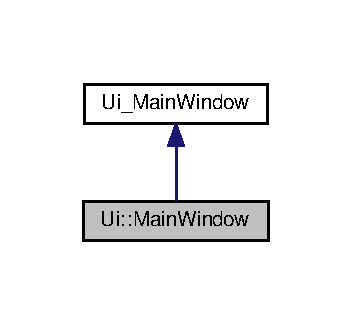
\includegraphics[width=169pt]{class_ui_1_1_main_window__inherit__graph}
\end{center}
\end{figure}


Collaboration diagram for Ui\+:\+:Main\+Window\+:\nopagebreak
\begin{figure}[H]
\begin{center}
\leavevmode
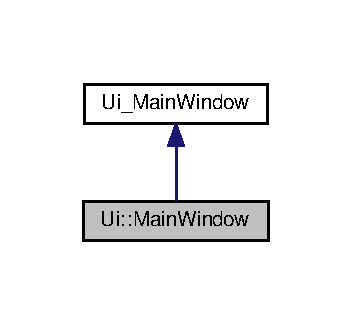
\includegraphics[width=169pt]{class_ui_1_1_main_window__coll__graph}
\end{center}
\end{figure}
\subsection*{Additional Inherited Members}


\subsection{Detailed Description}


The documentation for this class was generated from the following file\+:\begin{DoxyCompactItemize}
\item 
/home/jbs/catkin\+\_\+ws/src/traj\+\_\+gen\+\_\+vis\+\_\+developing/src/build-\/qt\+\_\+ui-\/\+Desktop-\/\+Debug/\hyperlink{ui__mainwindow_8h}{ui\+\_\+mainwindow.\+h}\end{DoxyCompactItemize}

\hypertarget{class_main_window}{}\section{Main\+Window Class Reference}
\label{class_main_window}\index{Main\+Window@{Main\+Window}}


{\ttfamily \#include $<$mainwindow.\+h$>$}



Inheritance diagram for Main\+Window\+:\nopagebreak
\begin{figure}[H]
\begin{center}
\leavevmode
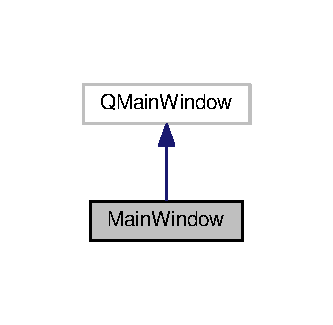
\includegraphics[width=160pt]{class_main_window__inherit__graph}
\end{center}
\end{figure}


Collaboration diagram for Main\+Window\+:
\nopagebreak
\begin{figure}[H]
\begin{center}
\leavevmode
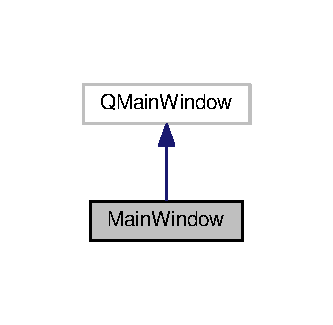
\includegraphics[width=350pt]{class_main_window__coll__graph}
\end{center}
\end{figure}
\subsection*{Public Member Functions}
\begin{DoxyCompactItemize}
\item 
\hyperlink{class_main_window_a6f0a90213d93b861d43c09dd01c52962}{Main\+Window} (\hyperlink{class_q_node}{Q\+Node} $\ast$\hyperlink{class_main_window_ac9d45be6e40fe6917339119e15c1b120}{qnode}, Q\+Widget $\ast$parent=0)
\item 
\hyperlink{class_main_window_ae98d00a93bc118200eeef9f9bba1dba7}{$\sim$\+Main\+Window} ()
\item 
void \hyperlink{class_main_window_a4e20a4a065fbb0e4d3532a45a0a91425}{close\+Event} (Q\+Close\+Event $\ast$event)
\item 
void \hyperlink{class_main_window_a4abba2c52f756524c0f388d0d3e6d6ec}{Read\+Settings} ()
\item 
void \hyperlink{class_main_window_a56a5e4d5e0a022e8c1ecf350d2916ade}{Write\+Settings} ()
\end{DoxyCompactItemize}
\subsection*{Private Slots}
\begin{DoxyCompactItemize}
\item 
void \hyperlink{class_main_window_a996e7b8e246db04a9931ea8c058eedf8}{on\+\_\+push\+Button\+\_\+chaser\+\_\+clicked} ()
\item 
void \hyperlink{class_main_window_a9aebdb686fc8f44bc84454443b094ef7}{on\+\_\+push\+Button\+\_\+ros\+\_\+clicked} ()
\item 
void \hyperlink{class_main_window_a543d311321e5dcb7a42384dd67c6bff4}{on\+\_\+push\+Button\+\_\+waypoint\+\_\+clicked} ()
\item 
void \hyperlink{class_main_window_a3cdeb477328d4aaeac315f62c632a4f2}{on\+\_\+push\+Button\+\_\+trajectory\+\_\+clicked} ()
\item 
void \hyperlink{class_main_window_aec26150ce3a1688a40230b79b088921d}{on\+\_\+push\+Button\+\_\+simulation\+\_\+clicked} ()
\item 
void \hyperlink{class_main_window_a5f2b259d7c85d5d32c1207a34d8b9af4}{on\+\_\+push\+Button\+\_\+save\+\_\+clicked} ()
\item 
void \hyperlink{class_main_window_a9c676468f012e842cd443d8029f8a242}{on\+\_\+push\+Button\+\_\+load\+\_\+clicked} ()
\item 
void \hyperlink{class_main_window_af777763ec745a8eeffe3f9925005fac1}{on\+\_\+push\+Button\+\_\+clear\+\_\+clicked} ()
\item 
void \hyperlink{class_main_window_a41e769472d468772dd3851cbd20ca9fb}{on\+\_\+push\+Button\+\_\+undo\+\_\+clicked} ()
\item 
void \hyperlink{class_main_window_a00ace1276164789fa5383e80ecbf8c6f}{on\+\_\+push\+Button\+\_\+one\+\_\+shot\+\_\+clicked} ()
\item 
void \hyperlink{class_main_window_a4513ffcd68256d01c44fa2602d4c6880}{text\+Edit\+\_\+write} (Q\+String)
\end{DoxyCompactItemize}
\subsection*{Private Attributes}
\begin{DoxyCompactItemize}
\item 
\hyperlink{class_ui_1_1_main_window}{Ui\+::\+Main\+Window} $\ast$ \hyperlink{class_main_window_a35466a70ed47252a0191168126a352a5}{ui}
\item 
\hyperlink{class_q_node}{Q\+Node} $\ast$ \hyperlink{class_main_window_ac9d45be6e40fe6917339119e15c1b120}{qnode}
\end{DoxyCompactItemize}


\subsection{Detailed Description}


\subsection{Constructor \& Destructor Documentation}
\index{Main\+Window@{Main\+Window}!Main\+Window@{Main\+Window}}
\index{Main\+Window@{Main\+Window}!Main\+Window@{Main\+Window}}
\subsubsection[{\texorpdfstring{Main\+Window(\+Q\+Node $\ast$qnode, Q\+Widget $\ast$parent=0)}{MainWindow(QNode *qnode, QWidget *parent=0)}}]{\setlength{\rightskip}{0pt plus 5cm}Main\+Window\+::\+Main\+Window (
\begin{DoxyParamCaption}
\item[{{\bf Q\+Node} $\ast$}]{qnode, }
\item[{Q\+Widget $\ast$}]{parent = {\ttfamily 0}}
\end{DoxyParamCaption}
)\hspace{0.3cm}{\ttfamily [explicit]}}\hypertarget{class_main_window_a6f0a90213d93b861d43c09dd01c52962}{}\label{class_main_window_a6f0a90213d93b861d43c09dd01c52962}

\begin{DoxyCode}
5                                                    :
6     QMainWindow(parent),\hyperlink{class_main_window_ac9d45be6e40fe6917339119e15c1b120}{qnode}(qnode),
7     \hyperlink{class_main_window_a35466a70ed47252a0191168126a352a5}{ui}(\textcolor{keyword}{new} \hyperlink{class_ui_1_1_main_window}{Ui::MainWindow})
8 \{
9     \hyperlink{class_main_window_a35466a70ed47252a0191168126a352a5}{ui}->\hyperlink{class_ui___main_window_acf4a0872c4c77d8f43a2ec66ed849b58}{setupUi}(\textcolor{keyword}{this});
10 
11 
12     \textcolor{comment}{// intial configuration}
13 
14     \textcolor{comment}{// logos}
15     \textcolor{keywordtype}{string} cd = \_\_FILE\_\_;
16     cd.erase(cd.end()-14,cd.end());
17     cout<<\textcolor{stringliteral}{"current directory: "}<<cd<<endl;
18 
19     QPixmap pix\_larr((cd + \textcolor{stringliteral}{"/resources/LARR.jpg"}).c\_str());
20     \textcolor{keywordtype}{int} w = \hyperlink{class_main_window_a35466a70ed47252a0191168126a352a5}{ui}->\hyperlink{class_ui___main_window_a32587f1e879f5b685d375d2daa20f7a6}{label\_larr}->width();
21     \textcolor{keywordtype}{int} h = \hyperlink{class_main_window_a35466a70ed47252a0191168126a352a5}{ui}->\hyperlink{class_ui___main_window_a32587f1e879f5b685d375d2daa20f7a6}{label\_larr}->height();
22     \hyperlink{class_main_window_a35466a70ed47252a0191168126a352a5}{ui}->\hyperlink{class_ui___main_window_a32587f1e879f5b685d375d2daa20f7a6}{label\_larr}->setPixmap(pix\_larr.scaled(w,h,Qt::KeepAspectRatio));
23 
24     QPixmap pix\_larr2((cd +\textcolor{stringliteral}{"/resources/maxresdefault.jpg"}).c\_str());
25     \textcolor{keywordtype}{int} w2 = \hyperlink{class_main_window_a35466a70ed47252a0191168126a352a5}{ui}->\hyperlink{class_ui___main_window_a06fc1a01ac3ba3d4d1f75a0e8ab06684}{label\_larr2}->width();
26     \textcolor{keywordtype}{int} h2 = \hyperlink{class_main_window_a35466a70ed47252a0191168126a352a5}{ui}->\hyperlink{class_ui___main_window_a06fc1a01ac3ba3d4d1f75a0e8ab06684}{label\_larr2}->height();
27     \hyperlink{class_main_window_a35466a70ed47252a0191168126a352a5}{ui}->\hyperlink{class_ui___main_window_a06fc1a01ac3ba3d4d1f75a0e8ab06684}{label\_larr2}->setPixmap(pix\_larr2.scaled(w2,h2,Qt::KeepAspectRatio));
28 
29     \textcolor{comment}{// checkable }
30     \hyperlink{class_main_window_a35466a70ed47252a0191168126a352a5}{ui}->\hyperlink{class_ui___main_window_afd109ead0ad1ae7ae67ad1df803c9c38}{pushButton\_simulation}->setStyleSheet(\textcolor{stringliteral}{"QPushButton:checked\{background-color:
       rgba(100, 20, 20,50); \}"});
31     
32     QObject::connect(qnode, SIGNAL(rosShutdown()), \textcolor{keyword}{this}, SLOT(close()));
33     QObject::connect(qnode,SIGNAL(writeOnBoard(QString)),\textcolor{keyword}{this},SLOT(
      \hyperlink{class_main_window_a4513ffcd68256d01c44fa2602d4c6880}{textEdit\_write}(QString)));
34 
35     \textcolor{comment}{// load settings }
36     \hyperlink{class_main_window_a4abba2c52f756524c0f388d0d3e6d6ec}{ReadSettings}();
37 
38 \}
\end{DoxyCode}
\index{Main\+Window@{Main\+Window}!````~Main\+Window@{$\sim$\+Main\+Window}}
\index{````~Main\+Window@{$\sim$\+Main\+Window}!Main\+Window@{Main\+Window}}
\subsubsection[{\texorpdfstring{$\sim$\+Main\+Window()}{~MainWindow()}}]{\setlength{\rightskip}{0pt plus 5cm}Main\+Window\+::$\sim$\+Main\+Window (
\begin{DoxyParamCaption}
{}
\end{DoxyParamCaption}
)}\hypertarget{class_main_window_ae98d00a93bc118200eeef9f9bba1dba7}{}\label{class_main_window_ae98d00a93bc118200eeef9f9bba1dba7}

\begin{DoxyCode}
41 \{
42     \textcolor{keyword}{delete} \hyperlink{class_main_window_a35466a70ed47252a0191168126a352a5}{ui};
43 \}
\end{DoxyCode}


\subsection{Member Function Documentation}
\index{Main\+Window@{Main\+Window}!close\+Event@{close\+Event}}
\index{close\+Event@{close\+Event}!Main\+Window@{Main\+Window}}
\subsubsection[{\texorpdfstring{close\+Event(\+Q\+Close\+Event $\ast$event)}{closeEvent(QCloseEvent *event)}}]{\setlength{\rightskip}{0pt plus 5cm}void Main\+Window\+::close\+Event (
\begin{DoxyParamCaption}
\item[{Q\+Close\+Event $\ast$}]{event}
\end{DoxyParamCaption}
)}\hypertarget{class_main_window_a4e20a4a065fbb0e4d3532a45a0a91425}{}\label{class_main_window_a4e20a4a065fbb0e4d3532a45a0a91425}

\begin{DoxyCode}
234                                              \{
235 
236         \hyperlink{class_main_window_ac9d45be6e40fe6917339119e15c1b120}{qnode}->\hyperlink{class_q_node_a770568addece696138f515d38408ff5c}{shutdown}();
237         \hyperlink{class_main_window_a56a5e4d5e0a022e8c1ecf350d2916ade}{WriteSettings}();
238         QMainWindow::closeEvent(event);
239 \}
\end{DoxyCode}
\index{Main\+Window@{Main\+Window}!on\+\_\+push\+Button\+\_\+chaser\+\_\+clicked@{on\+\_\+push\+Button\+\_\+chaser\+\_\+clicked}}
\index{on\+\_\+push\+Button\+\_\+chaser\+\_\+clicked@{on\+\_\+push\+Button\+\_\+chaser\+\_\+clicked}!Main\+Window@{Main\+Window}}
\subsubsection[{\texorpdfstring{on\+\_\+push\+Button\+\_\+chaser\+\_\+clicked}{on_pushButton_chaser_clicked}}]{\setlength{\rightskip}{0pt plus 5cm}void Main\+Window\+::on\+\_\+push\+Button\+\_\+chaser\+\_\+clicked (
\begin{DoxyParamCaption}
{}
\end{DoxyParamCaption}
)\hspace{0.3cm}{\ttfamily [private]}, {\ttfamily [slot]}}\hypertarget{class_main_window_a996e7b8e246db04a9931ea8c058eedf8}{}\label{class_main_window_a996e7b8e246db04a9931ea8c058eedf8}

\begin{DoxyCode}
70                                              \{
71 
72     \textcolor{keywordflow}{if}(\hyperlink{class_main_window_a35466a70ed47252a0191168126a352a5}{ui}->\hyperlink{class_ui___main_window_a9e8499b7c9a9717499abde993da72ed5}{pushButton\_chaser}->isChecked())\{      
73         \hyperlink{class_main_window_ac9d45be6e40fe6917339119e15c1b120}{qnode}->\hyperlink{class_q_node_ad2d828488fb632a008c7d3ee0e1d1fa2}{chaser\_wrapper}.\hyperlink{class_wrapper_a8cddd5ffbaeb5ab0b5d8d8d0c74f810f}{objects\_handler}.
      \hyperlink{class_objects_handler_acaefe98eb412d4c32cda2bf0bd602ae7}{is\_insert\_permit} = \textcolor{keyword}{true};  
74         \hyperlink{class_main_window_a35466a70ed47252a0191168126a352a5}{ui}->\hyperlink{class_ui___main_window_af13441b9fd874f1aeb2ec5cefaeb0bce}{textEdit\_board}->append(\textcolor{stringliteral}{"please select chaser init pose: /chaser\_init\_pose"});
75     \}\textcolor{keywordflow}{else}\{
76         \hyperlink{class_main_window_a35466a70ed47252a0191168126a352a5}{ui}->\hyperlink{class_ui___main_window_af13441b9fd874f1aeb2ec5cefaeb0bce}{textEdit\_board}->append(\textcolor{stringliteral}{"finishing chaser spawning selection"});
77         \hyperlink{class_main_window_ac9d45be6e40fe6917339119e15c1b120}{qnode}->\hyperlink{class_q_node_ad2d828488fb632a008c7d3ee0e1d1fa2}{chaser\_wrapper}.\hyperlink{class_wrapper_a8cddd5ffbaeb5ab0b5d8d8d0c74f810f}{objects\_handler}.
      \hyperlink{class_objects_handler_acaefe98eb412d4c32cda2bf0bd602ae7}{is\_insert\_permit} = \textcolor{keyword}{false};  
78 
79     \}
80 
81 \}
\end{DoxyCode}
\index{Main\+Window@{Main\+Window}!on\+\_\+push\+Button\+\_\+clear\+\_\+clicked@{on\+\_\+push\+Button\+\_\+clear\+\_\+clicked}}
\index{on\+\_\+push\+Button\+\_\+clear\+\_\+clicked@{on\+\_\+push\+Button\+\_\+clear\+\_\+clicked}!Main\+Window@{Main\+Window}}
\subsubsection[{\texorpdfstring{on\+\_\+push\+Button\+\_\+clear\+\_\+clicked}{on_pushButton_clear_clicked}}]{\setlength{\rightskip}{0pt plus 5cm}void Main\+Window\+::on\+\_\+push\+Button\+\_\+clear\+\_\+clicked (
\begin{DoxyParamCaption}
{}
\end{DoxyParamCaption}
)\hspace{0.3cm}{\ttfamily [private]}, {\ttfamily [slot]}}\hypertarget{class_main_window_af777763ec745a8eeffe3f9925005fac1}{}\label{class_main_window_af777763ec745a8eeffe3f9925005fac1}

\begin{DoxyCode}
181 \{
182     \hyperlink{class_main_window_ac9d45be6e40fe6917339119e15c1b120}{qnode}->\hyperlink{class_q_node_adc66765125dfd755d5e7f0c0eb6e6395}{target\_manager}.\hyperlink{class_target_manager_a13242c4a8b96b97cfeddea19aabc1181}{clear\_waypoint}();
183 \}
\end{DoxyCode}
\index{Main\+Window@{Main\+Window}!on\+\_\+push\+Button\+\_\+load\+\_\+clicked@{on\+\_\+push\+Button\+\_\+load\+\_\+clicked}}
\index{on\+\_\+push\+Button\+\_\+load\+\_\+clicked@{on\+\_\+push\+Button\+\_\+load\+\_\+clicked}!Main\+Window@{Main\+Window}}
\subsubsection[{\texorpdfstring{on\+\_\+push\+Button\+\_\+load\+\_\+clicked}{on_pushButton_load_clicked}}]{\setlength{\rightskip}{0pt plus 5cm}void Main\+Window\+::on\+\_\+push\+Button\+\_\+load\+\_\+clicked (
\begin{DoxyParamCaption}
{}
\end{DoxyParamCaption}
)\hspace{0.3cm}{\ttfamily [private]}, {\ttfamily [slot]}}\hypertarget{class_main_window_a9c676468f012e842cd443d8029f8a242}{}\label{class_main_window_a9c676468f012e842cd443d8029f8a242}

\begin{DoxyCode}
137 \{
138     \textcolor{comment}{// file read : queue wil be filled with these}
139 
140     \textcolor{keywordtype}{string} filename = \hyperlink{class_main_window_a35466a70ed47252a0191168126a352a5}{ui}->\hyperlink{class_ui___main_window_a4a75bfb754049f89fccef822cad712d6}{lineEdit\_target\_trajectory}->text().toStdString();
141     std::ifstream infile;
142     infile.open(filename);
143     \textcolor{keywordflow}{if}(infile.is\_open())
144         \hyperlink{class_main_window_a35466a70ed47252a0191168126a352a5}{ui}->\hyperlink{class_ui___main_window_af13441b9fd874f1aeb2ec5cefaeb0bce}{textEdit\_board}->append(QString(\textcolor{stringliteral}{"pnts reading.."}));
145     \textcolor{keywordflow}{else}
146     \{
147         \hyperlink{class_main_window_a35466a70ed47252a0191168126a352a5}{ui}->\hyperlink{class_ui___main_window_af13441b9fd874f1aeb2ec5cefaeb0bce}{textEdit\_board}->append(QString(\textcolor{stringliteral}{"could not open file."}));
148         \textcolor{keywordflow}{return};
149     \}
150 
151     std::vector<geometry\_msgs::PoseStamped> queue\_replace;
152 
153     \textcolor{keywordflow}{while} (! infile.eof())\{
154         std::string line;
155         getline(infile, line); \textcolor{comment}{// if no delimiter given, new line is that}
156         \textcolor{comment}{// std::cout<<line<<std::endl;}
157         std::stringstream stream(line);
158         std::string val;
159         \textcolor{keywordtype}{int} xyz\_idx = 0;
160         geometry\_msgs::PoseStamped wpnt;
161 
162         \textcolor{keywordflow}{while}(! stream.eof()) \{
163             getline(stream, val, \textcolor{charliteral}{','});
164             \textcolor{keywordflow}{if}(xyz\_idx == 0)
165                 wpnt.pose.position.x = atof(val.c\_str());
166             \textcolor{keywordflow}{else} \textcolor{keywordflow}{if}(xyz\_idx == 1)
167                 wpnt.pose.position.y = atof(val.c\_str());
168             \textcolor{keywordflow}{else}
169                 wpnt.pose.position.z = atof(val.c\_str());
170             xyz\_idx ++;
171         \}
172         queue\_replace.push\_back(wpnt);
173         \textcolor{comment}{// std::cout<< wpnt.pose.position.x <<" , "<< wpnt.pose.position.y <<" ,
       "<<wpnt.pose.position.z<<std::endl;}
174     \}
175 
176     queue\_replace.pop\_back();
177     \hyperlink{class_main_window_ac9d45be6e40fe6917339119e15c1b120}{qnode}->\hyperlink{class_q_node_adc66765125dfd755d5e7f0c0eb6e6395}{target\_manager}.\hyperlink{class_target_manager_a8b96689879cecac3d9109914eb6230ef}{queue\_file\_load}(queue\_replace);
178 \}
\end{DoxyCode}
\index{Main\+Window@{Main\+Window}!on\+\_\+push\+Button\+\_\+one\+\_\+shot\+\_\+clicked@{on\+\_\+push\+Button\+\_\+one\+\_\+shot\+\_\+clicked}}
\index{on\+\_\+push\+Button\+\_\+one\+\_\+shot\+\_\+clicked@{on\+\_\+push\+Button\+\_\+one\+\_\+shot\+\_\+clicked}!Main\+Window@{Main\+Window}}
\subsubsection[{\texorpdfstring{on\+\_\+push\+Button\+\_\+one\+\_\+shot\+\_\+clicked}{on_pushButton_one_shot_clicked}}]{\setlength{\rightskip}{0pt plus 5cm}void Main\+Window\+::on\+\_\+push\+Button\+\_\+one\+\_\+shot\+\_\+clicked (
\begin{DoxyParamCaption}
{}
\end{DoxyParamCaption}
)\hspace{0.3cm}{\ttfamily [private]}, {\ttfamily [slot]}}\hypertarget{class_main_window_a00ace1276164789fa5383e80ecbf8c6f}{}\label{class_main_window_a00ace1276164789fa5383e80ecbf8c6f}

\begin{DoxyCode}
190                                                \{
191     \hyperlink{class_main_window_a35466a70ed47252a0191168126a352a5}{ui}->\hyperlink{class_ui___main_window_af13441b9fd874f1aeb2ec5cefaeb0bce}{textEdit\_board}->append(\textcolor{stringliteral}{"one shot simulatoin requested."});
192     \textcolor{keywordtype}{double} tf = atoi(\hyperlink{class_main_window_a35466a70ed47252a0191168126a352a5}{ui}->\hyperlink{class_ui___main_window_afc0d94ce5096c619c413cfae9b62014c}{lineEdit\_tf}->text().toStdString().c\_str());    
193     \textcolor{keywordflow}{if} (\hyperlink{class_main_window_ac9d45be6e40fe6917339119e15c1b120}{qnode}->\hyperlink{class_q_node_a65f0fc9f27f336150f33b53a7c51d80b}{trigger\_one\_shot}(tf))
194         \hyperlink{class_main_window_a35466a70ed47252a0191168126a352a5}{ui}->\hyperlink{class_ui___main_window_af13441b9fd874f1aeb2ec5cefaeb0bce}{textEdit\_board}->append(\textcolor{stringliteral}{"chasing path obtained"});
195     \textcolor{keywordflow}{else} 
196         \hyperlink{class_main_window_a35466a70ed47252a0191168126a352a5}{ui}->\hyperlink{class_ui___main_window_af13441b9fd874f1aeb2ec5cefaeb0bce}{textEdit\_board}->append(\textcolor{stringliteral}{"chasing failed"});    
197 \};
\end{DoxyCode}
\index{Main\+Window@{Main\+Window}!on\+\_\+push\+Button\+\_\+ros\+\_\+clicked@{on\+\_\+push\+Button\+\_\+ros\+\_\+clicked}}
\index{on\+\_\+push\+Button\+\_\+ros\+\_\+clicked@{on\+\_\+push\+Button\+\_\+ros\+\_\+clicked}!Main\+Window@{Main\+Window}}
\subsubsection[{\texorpdfstring{on\+\_\+push\+Button\+\_\+ros\+\_\+clicked}{on_pushButton_ros_clicked}}]{\setlength{\rightskip}{0pt plus 5cm}void Main\+Window\+::on\+\_\+push\+Button\+\_\+ros\+\_\+clicked (
\begin{DoxyParamCaption}
{}
\end{DoxyParamCaption}
)\hspace{0.3cm}{\ttfamily [private]}, {\ttfamily [slot]}}\hypertarget{class_main_window_a9aebdb686fc8f44bc84454443b094ef7}{}\label{class_main_window_a9aebdb686fc8f44bc84454443b094ef7}

\begin{DoxyCode}
46 \{
47     \textcolor{keywordflow}{if}(\hyperlink{class_main_window_ac9d45be6e40fe6917339119e15c1b120}{qnode}->\hyperlink{class_q_node_a32d00dbcf15c277e08caabf95af04f6e}{on\_init}())\{
48         \hyperlink{class_main_window_a35466a70ed47252a0191168126a352a5}{ui}->\hyperlink{class_ui___main_window_af13441b9fd874f1aeb2ec5cefaeb0bce}{textEdit\_board}->append(\textcolor{stringliteral}{"ros connected."});
49         \hyperlink{class_main_window_ac9d45be6e40fe6917339119e15c1b120}{qnode}->\hyperlink{class_q_node_a98b08e7704b00df8648f8c08dffe950c}{is\_connected} = \textcolor{keyword}{true};
50 
51     \}\textcolor{keywordflow}{else}\{
52         \hyperlink{class_main_window_a35466a70ed47252a0191168126a352a5}{ui}->\hyperlink{class_ui___main_window_af13441b9fd874f1aeb2ec5cefaeb0bce}{textEdit\_board}->append(\textcolor{stringliteral}{"failed. retry"});
53     \}
54 \}
\end{DoxyCode}
\index{Main\+Window@{Main\+Window}!on\+\_\+push\+Button\+\_\+save\+\_\+clicked@{on\+\_\+push\+Button\+\_\+save\+\_\+clicked}}
\index{on\+\_\+push\+Button\+\_\+save\+\_\+clicked@{on\+\_\+push\+Button\+\_\+save\+\_\+clicked}!Main\+Window@{Main\+Window}}
\subsubsection[{\texorpdfstring{on\+\_\+push\+Button\+\_\+save\+\_\+clicked}{on_pushButton_save_clicked}}]{\setlength{\rightskip}{0pt plus 5cm}void Main\+Window\+::on\+\_\+push\+Button\+\_\+save\+\_\+clicked (
\begin{DoxyParamCaption}
{}
\end{DoxyParamCaption}
)\hspace{0.3cm}{\ttfamily [private]}, {\ttfamily [slot]}}\hypertarget{class_main_window_a5f2b259d7c85d5d32c1207a34d8b9af4}{}\label{class_main_window_a5f2b259d7c85d5d32c1207a34d8b9af4}

\begin{DoxyCode}
115 \{
116 
117     \textcolor{comment}{// file write}
118     std::ofstream wnpt\_file;
119     \textcolor{keywordtype}{string} filename = \hyperlink{class_main_window_a35466a70ed47252a0191168126a352a5}{ui}->\hyperlink{class_ui___main_window_a4a75bfb754049f89fccef822cad712d6}{lineEdit\_target\_trajectory}->text().toStdString();
120     wnpt\_file.open(filename);
121 
122     \textcolor{keywordflow}{if}(wnpt\_file.is\_open())\{
123         \textcolor{keywordflow}{for}(\textcolor{keyword}{auto} it = \hyperlink{class_main_window_ac9d45be6e40fe6917339119e15c1b120}{qnode}->\hyperlink{class_q_node_adc66765125dfd755d5e7f0c0eb6e6395}{target\_manager}.\hyperlink{class_target_manager_a0bbcb1981504e3bc587c3a98f41a91e9}{queue}.begin();it<
      \hyperlink{class_main_window_ac9d45be6e40fe6917339119e15c1b120}{qnode}->\hyperlink{class_q_node_adc66765125dfd755d5e7f0c0eb6e6395}{target\_manager}.\hyperlink{class_target_manager_a0bbcb1981504e3bc587c3a98f41a91e9}{queue}.end();it++)\{
124             wnpt\_file<<std::to\_string(it->pose.position.x)<<\textcolor{stringliteral}{","}<<std::to\_string(it->pose.position.y)<<\textcolor{stringliteral}{","}<<
      std::to\_string(it->pose.position.z)<<\textcolor{stringliteral}{"\(\backslash\)n"};
125         \}
126         wnpt\_file.close();
127 
128         
129         \hyperlink{class_main_window_a35466a70ed47252a0191168126a352a5}{ui}->\hyperlink{class_ui___main_window_af13441b9fd874f1aeb2ec5cefaeb0bce}{textEdit\_board}->append(QString((\textcolor{keywordtype}{string}(\textcolor{stringliteral}{"to "}) + 
      \hyperlink{_common_8h_a7770cb36d4f4c6e78ff68516ecb2123c}{GetCurrentWorkingDir}()+\textcolor{stringliteral}{"/"} + filename + \textcolor{keywordtype}{string}(\textcolor{stringliteral}{", written"})).data()));
130 
131     \}\textcolor{keywordflow}{else}
132         \hyperlink{class_main_window_a35466a70ed47252a0191168126a352a5}{ui}->\hyperlink{class_ui___main_window_af13441b9fd874f1aeb2ec5cefaeb0bce}{textEdit\_board}->append(QString(\textcolor{stringliteral}{"file not written."}));
133 
134 \}
\end{DoxyCode}
\index{Main\+Window@{Main\+Window}!on\+\_\+push\+Button\+\_\+simulation\+\_\+clicked@{on\+\_\+push\+Button\+\_\+simulation\+\_\+clicked}}
\index{on\+\_\+push\+Button\+\_\+simulation\+\_\+clicked@{on\+\_\+push\+Button\+\_\+simulation\+\_\+clicked}!Main\+Window@{Main\+Window}}
\subsubsection[{\texorpdfstring{on\+\_\+push\+Button\+\_\+simulation\+\_\+clicked}{on_pushButton_simulation_clicked}}]{\setlength{\rightskip}{0pt plus 5cm}void Main\+Window\+::on\+\_\+push\+Button\+\_\+simulation\+\_\+clicked (
\begin{DoxyParamCaption}
{}
\end{DoxyParamCaption}
)\hspace{0.3cm}{\ttfamily [private]}, {\ttfamily [slot]}}\hypertarget{class_main_window_aec26150ce3a1688a40230b79b088921d}{}\label{class_main_window_aec26150ce3a1688a40230b79b088921d}

\begin{DoxyCode}
94 \{
95     \textcolor{keywordflow}{if}(\hyperlink{class_main_window_a35466a70ed47252a0191168126a352a5}{ui}->\hyperlink{class_ui___main_window_afd109ead0ad1ae7ae67ad1df803c9c38}{pushButton\_simulation}->isChecked())\{ 
96 
97         \textcolor{keywordflow}{if}(\hyperlink{class_main_window_ac9d45be6e40fe6917339119e15c1b120}{qnode}->\hyperlink{class_q_node_ad2d828488fb632a008c7d3ee0e1d1fa2}{chaser\_wrapper}.\hyperlink{class_wrapper_a8cddd5ffbaeb5ab0b5d8d8d0c74f810f}{objects\_handler}.
      \hyperlink{class_objects_handler_a16165ae7c0167ba8d2a0151a8a4fbfd5}{is\_chaser\_spawned} and \hyperlink{class_main_window_ac9d45be6e40fe6917339119e15c1b120}{qnode}->\hyperlink{class_q_node_adc66765125dfd755d5e7f0c0eb6e6395}{target\_manager}.
      \hyperlink{class_target_manager_a507af7ce1ac562510c1b907553a2e596}{is\_path})\{
98             \hyperlink{class_main_window_a35466a70ed47252a0191168126a352a5}{ui}->\hyperlink{class_ui___main_window_af13441b9fd874f1aeb2ec5cefaeb0bce}{textEdit\_board}->append(\textcolor{stringliteral}{"move target.."});
99             \textcolor{comment}{// simulation end time }
100             \hyperlink{class_main_window_ac9d45be6e40fe6917339119e15c1b120}{qnode}->\hyperlink{class_q_node_a7a127726e48aa5bde733d715af7a744c}{simulation\_end\_time} = atof(\hyperlink{class_main_window_a35466a70ed47252a0191168126a352a5}{ui}->
      \hyperlink{class_ui___main_window_afc0d94ce5096c619c413cfae9b62014c}{lineEdit\_tf}->text().toStdString().c\_str());
101             \hyperlink{class_main_window_ac9d45be6e40fe6917339119e15c1b120}{qnode}->\hyperlink{class_q_node_a6ace2d0aa89adecfe699b3f1c3ce0b0f}{is\_in\_session} = \textcolor{keyword}{true};
102             \hyperlink{class_main_window_ac9d45be6e40fe6917339119e15c1b120}{qnode}->\hyperlink{class_q_node_a96e6599c14732ded065ae6a5b004f872}{button\_click\_time} = ros::Time::now();        
103         \}
104         \textcolor{keywordflow}{else}\{
105             \hyperlink{class_main_window_a35466a70ed47252a0191168126a352a5}{ui}->\hyperlink{class_ui___main_window_af13441b9fd874f1aeb2ec5cefaeb0bce}{textEdit\_board}->append(\textcolor{stringliteral}{"target path not obtained or no chaser spawned."});
106         \}
107     \}\textcolor{keywordflow}{else}\{
108         \hyperlink{class_main_window_a35466a70ed47252a0191168126a352a5}{ui}->\hyperlink{class_ui___main_window_af13441b9fd874f1aeb2ec5cefaeb0bce}{textEdit\_board}->append(\textcolor{stringliteral}{"stop target."});
109         \hyperlink{class_main_window_ac9d45be6e40fe6917339119e15c1b120}{qnode}->\hyperlink{class_q_node_a6ace2d0aa89adecfe699b3f1c3ce0b0f}{is\_in\_session} = \textcolor{keyword}{false};
110         \hyperlink{class_main_window_ac9d45be6e40fe6917339119e15c1b120}{qnode}->\hyperlink{class_q_node_a4b5f0a40821fbb176de620cb5a3921f7}{previous\_elapsed} = (ros::Time::now() - \hyperlink{class_main_window_ac9d45be6e40fe6917339119e15c1b120}{qnode}->
      \hyperlink{class_q_node_a96e6599c14732ded065ae6a5b004f872}{button\_click\_time}).toSec() + \hyperlink{class_main_window_ac9d45be6e40fe6917339119e15c1b120}{qnode}->\hyperlink{class_q_node_a4b5f0a40821fbb176de620cb5a3921f7}{previous\_elapsed}; \textcolor{comment}{// total
       elasped time}
111     \}
112 \}
\end{DoxyCode}
\index{Main\+Window@{Main\+Window}!on\+\_\+push\+Button\+\_\+trajectory\+\_\+clicked@{on\+\_\+push\+Button\+\_\+trajectory\+\_\+clicked}}
\index{on\+\_\+push\+Button\+\_\+trajectory\+\_\+clicked@{on\+\_\+push\+Button\+\_\+trajectory\+\_\+clicked}!Main\+Window@{Main\+Window}}
\subsubsection[{\texorpdfstring{on\+\_\+push\+Button\+\_\+trajectory\+\_\+clicked}{on_pushButton_trajectory_clicked}}]{\setlength{\rightskip}{0pt plus 5cm}void Main\+Window\+::on\+\_\+push\+Button\+\_\+trajectory\+\_\+clicked (
\begin{DoxyParamCaption}
{}
\end{DoxyParamCaption}
)\hspace{0.3cm}{\ttfamily [private]}, {\ttfamily [slot]}}\hypertarget{class_main_window_a3cdeb477328d4aaeac315f62c632a4f2}{}\label{class_main_window_a3cdeb477328d4aaeac315f62c632a4f2}

\begin{DoxyCode}
84 \{
85     
86     \textcolor{keywordtype}{double} tf = atof(\hyperlink{class_main_window_a35466a70ed47252a0191168126a352a5}{ui}->\hyperlink{class_ui___main_window_afc0d94ce5096c619c413cfae9b62014c}{lineEdit\_tf}->text().toStdString().c\_str());
87     \textcolor{keywordflow}{if}(\hyperlink{class_main_window_ac9d45be6e40fe6917339119e15c1b120}{qnode}->\hyperlink{class_q_node_adc66765125dfd755d5e7f0c0eb6e6395}{target\_manager}.\hyperlink{class_target_manager_a1c0e48d7a623e8b7caa11c6b1832956b}{global\_path\_generate}(tf))
88         \hyperlink{class_main_window_a4513ffcd68256d01c44fa2602d4c6880}{textEdit\_write}(\textcolor{stringliteral}{"target trajectory obtainted"});
89     \textcolor{keywordflow}{else}
90         \hyperlink{class_main_window_a4513ffcd68256d01c44fa2602d4c6880}{textEdit\_write}(\textcolor{stringliteral}{"target trajectory failed"});    
91 \}
\end{DoxyCode}
\index{Main\+Window@{Main\+Window}!on\+\_\+push\+Button\+\_\+undo\+\_\+clicked@{on\+\_\+push\+Button\+\_\+undo\+\_\+clicked}}
\index{on\+\_\+push\+Button\+\_\+undo\+\_\+clicked@{on\+\_\+push\+Button\+\_\+undo\+\_\+clicked}!Main\+Window@{Main\+Window}}
\subsubsection[{\texorpdfstring{on\+\_\+push\+Button\+\_\+undo\+\_\+clicked}{on_pushButton_undo_clicked}}]{\setlength{\rightskip}{0pt plus 5cm}void Main\+Window\+::on\+\_\+push\+Button\+\_\+undo\+\_\+clicked (
\begin{DoxyParamCaption}
{}
\end{DoxyParamCaption}
)\hspace{0.3cm}{\ttfamily [private]}, {\ttfamily [slot]}}\hypertarget{class_main_window_a41e769472d468772dd3851cbd20ca9fb}{}\label{class_main_window_a41e769472d468772dd3851cbd20ca9fb}

\begin{DoxyCode}
186 \{
187     \hyperlink{class_main_window_ac9d45be6e40fe6917339119e15c1b120}{qnode}->\hyperlink{class_q_node_adc66765125dfd755d5e7f0c0eb6e6395}{target\_manager}.\hyperlink{class_target_manager_af362d78ae6b0cc0a3ea288b2c138f482}{pop\_waypoint}();
188 \};
\end{DoxyCode}
\index{Main\+Window@{Main\+Window}!on\+\_\+push\+Button\+\_\+waypoint\+\_\+clicked@{on\+\_\+push\+Button\+\_\+waypoint\+\_\+clicked}}
\index{on\+\_\+push\+Button\+\_\+waypoint\+\_\+clicked@{on\+\_\+push\+Button\+\_\+waypoint\+\_\+clicked}!Main\+Window@{Main\+Window}}
\subsubsection[{\texorpdfstring{on\+\_\+push\+Button\+\_\+waypoint\+\_\+clicked}{on_pushButton_waypoint_clicked}}]{\setlength{\rightskip}{0pt plus 5cm}void Main\+Window\+::on\+\_\+push\+Button\+\_\+waypoint\+\_\+clicked (
\begin{DoxyParamCaption}
{}
\end{DoxyParamCaption}
)\hspace{0.3cm}{\ttfamily [private]}, {\ttfamily [slot]}}\hypertarget{class_main_window_a543d311321e5dcb7a42384dd67c6bff4}{}\label{class_main_window_a543d311321e5dcb7a42384dd67c6bff4}

\begin{DoxyCode}
57 \{
58     \textcolor{keywordflow}{if}(\hyperlink{class_main_window_a35466a70ed47252a0191168126a352a5}{ui}->\hyperlink{class_ui___main_window_a6b5d7c0f96cdb3276a33746fbcd7e8c7}{pushButton\_waypoint}->isChecked())\{        
59         \hyperlink{class_main_window_a35466a70ed47252a0191168126a352a5}{ui}->\hyperlink{class_ui___main_window_af13441b9fd874f1aeb2ec5cefaeb0bce}{textEdit\_board}->append(\textcolor{stringliteral}{"please select waypoints : /target\_waypoints "});
60         \hyperlink{class_main_window_ac9d45be6e40fe6917339119e15c1b120}{qnode}->\hyperlink{class_q_node_adc66765125dfd755d5e7f0c0eb6e6395}{target\_manager}.\hyperlink{class_target_manager_adf8a01c0942c3aac0445403d8f0f4cce}{is\_insert\_permit} = \textcolor{keyword}{true};
61 
62     \}\textcolor{keywordflow}{else}\{
63 
64         \hyperlink{class_main_window_a35466a70ed47252a0191168126a352a5}{ui}->\hyperlink{class_ui___main_window_af13441b9fd874f1aeb2ec5cefaeb0bce}{textEdit\_board}->append(\textcolor{stringliteral}{"finishing waypoints selection"});
65         \hyperlink{class_main_window_ac9d45be6e40fe6917339119e15c1b120}{qnode}->\hyperlink{class_q_node_adc66765125dfd755d5e7f0c0eb6e6395}{target\_manager}.\hyperlink{class_target_manager_adf8a01c0942c3aac0445403d8f0f4cce}{is\_insert\_permit} = \textcolor{keyword}{false};
66     \}
67 
68 \}
\end{DoxyCode}
\index{Main\+Window@{Main\+Window}!Read\+Settings@{Read\+Settings}}
\index{Read\+Settings@{Read\+Settings}!Main\+Window@{Main\+Window}}
\subsubsection[{\texorpdfstring{Read\+Settings()}{ReadSettings()}}]{\setlength{\rightskip}{0pt plus 5cm}void Main\+Window\+::\+Read\+Settings (
\begin{DoxyParamCaption}
{}
\end{DoxyParamCaption}
)}\hypertarget{class_main_window_a4abba2c52f756524c0f388d0d3e6d6ec}{}\label{class_main_window_a4abba2c52f756524c0f388d0d3e6d6ec}

\begin{DoxyCode}
204                              \{
205     QSettings settings(\textcolor{stringliteral}{"auto\_chaser"}, \hyperlink{class_main_window_ac9d45be6e40fe6917339119e15c1b120}{qnode}->\hyperlink{class_q_node_ac21ae24311df97ac0e15c97179763b0e}{nodeName}().c\_str());
206 
207     \textcolor{comment}{// setting names    }
208     QString filename\_logging = settings.value(\textcolor{stringliteral}{"filename\_logging"},QString(\textcolor{stringliteral}{"path\_saved.txt"})).toString();
209     QString filename\_waypoints = settings.value(\textcolor{stringliteral}{"filename\_waypoints"},QString(\textcolor{stringliteral}{"path\_saved.txt"})).toString();
210     QString simulation\_tf = settings.value(\textcolor{stringliteral}{"tf"}, QString(\textcolor{stringliteral}{"20"})).toString();
211 
212     
213     \textcolor{comment}{// fill with previous settings }
214     \hyperlink{class_main_window_a35466a70ed47252a0191168126a352a5}{ui}->\hyperlink{class_ui___main_window_a7ab71242b81ef9d13f83c16f6328f35d}{lineEdit\_logging\_dir}->setText(filename\_logging);
215     \hyperlink{class_main_window_a35466a70ed47252a0191168126a352a5}{ui}->\hyperlink{class_ui___main_window_afc0d94ce5096c619c413cfae9b62014c}{lineEdit\_tf}->setText(simulation\_tf);
216     \hyperlink{class_main_window_a35466a70ed47252a0191168126a352a5}{ui}->\hyperlink{class_ui___main_window_a4a75bfb754049f89fccef822cad712d6}{lineEdit\_target\_trajectory}->setText(filename\_waypoints);
217     
218 \}
\end{DoxyCode}
\index{Main\+Window@{Main\+Window}!text\+Edit\+\_\+write@{text\+Edit\+\_\+write}}
\index{text\+Edit\+\_\+write@{text\+Edit\+\_\+write}!Main\+Window@{Main\+Window}}
\subsubsection[{\texorpdfstring{text\+Edit\+\_\+write}{textEdit_write}}]{\setlength{\rightskip}{0pt plus 5cm}void Main\+Window\+::text\+Edit\+\_\+write (
\begin{DoxyParamCaption}
\item[{Q\+String}]{line}
\end{DoxyParamCaption}
)\hspace{0.3cm}{\ttfamily [private]}, {\ttfamily [slot]}}\hypertarget{class_main_window_a4513ffcd68256d01c44fa2602d4c6880}{}\label{class_main_window_a4513ffcd68256d01c44fa2602d4c6880}

\begin{DoxyCode}
199                                            \{    
200     \hyperlink{class_main_window_a35466a70ed47252a0191168126a352a5}{ui}->\hyperlink{class_ui___main_window_af13441b9fd874f1aeb2ec5cefaeb0bce}{textEdit\_board}->append(line);
201 \};
\end{DoxyCode}
\index{Main\+Window@{Main\+Window}!Write\+Settings@{Write\+Settings}}
\index{Write\+Settings@{Write\+Settings}!Main\+Window@{Main\+Window}}
\subsubsection[{\texorpdfstring{Write\+Settings()}{WriteSettings()}}]{\setlength{\rightskip}{0pt plus 5cm}void Main\+Window\+::\+Write\+Settings (
\begin{DoxyParamCaption}
{}
\end{DoxyParamCaption}
)}\hypertarget{class_main_window_a56a5e4d5e0a022e8c1ecf350d2916ade}{}\label{class_main_window_a56a5e4d5e0a022e8c1ecf350d2916ade}

\begin{DoxyCode}
220                               \{
221 
222     QSettings settings(\textcolor{stringliteral}{"auto\_chaser"}, \hyperlink{class_main_window_ac9d45be6e40fe6917339119e15c1b120}{qnode}->\hyperlink{class_q_node_ac21ae24311df97ac0e15c97179763b0e}{nodeName}().c\_str());
223     
224     settings.setValue(\textcolor{stringliteral}{"geometry"}, geometry());
225     settings.setValue(\textcolor{stringliteral}{"windowState"}, saveState());
226 
227     settings.setValue(\textcolor{stringliteral}{"filename\_logging"},\hyperlink{class_main_window_a35466a70ed47252a0191168126a352a5}{ui}->\hyperlink{class_ui___main_window_a7ab71242b81ef9d13f83c16f6328f35d}{lineEdit\_logging\_dir}->text());
228     settings.setValue(\textcolor{stringliteral}{"tf"},\hyperlink{class_main_window_a35466a70ed47252a0191168126a352a5}{ui}->\hyperlink{class_ui___main_window_afc0d94ce5096c619c413cfae9b62014c}{lineEdit\_tf}->text());
229     settings.setValue(\textcolor{stringliteral}{"filename\_waypoints"},\hyperlink{class_main_window_a35466a70ed47252a0191168126a352a5}{ui}->\hyperlink{class_ui___main_window_a4a75bfb754049f89fccef822cad712d6}{lineEdit\_target\_trajectory}->text
      ());
230 
231 
232 \}
\end{DoxyCode}


\subsection{Member Data Documentation}
\index{Main\+Window@{Main\+Window}!qnode@{qnode}}
\index{qnode@{qnode}!Main\+Window@{Main\+Window}}
\subsubsection[{\texorpdfstring{qnode}{qnode}}]{\setlength{\rightskip}{0pt plus 5cm}{\bf Q\+Node}$\ast$ Main\+Window\+::qnode\hspace{0.3cm}{\ttfamily [private]}}\hypertarget{class_main_window_ac9d45be6e40fe6917339119e15c1b120}{}\label{class_main_window_ac9d45be6e40fe6917339119e15c1b120}
\index{Main\+Window@{Main\+Window}!ui@{ui}}
\index{ui@{ui}!Main\+Window@{Main\+Window}}
\subsubsection[{\texorpdfstring{ui}{ui}}]{\setlength{\rightskip}{0pt plus 5cm}{\bf Ui\+::\+Main\+Window}$\ast$ Main\+Window\+::ui\hspace{0.3cm}{\ttfamily [private]}}\hypertarget{class_main_window_a35466a70ed47252a0191168126a352a5}{}\label{class_main_window_a35466a70ed47252a0191168126a352a5}


The documentation for this class was generated from the following files\+:\begin{DoxyCompactItemize}
\item 
/home/jbs/catkin\+\_\+ws/src/traj\+\_\+gen\+\_\+vis\+\_\+developing/src/qt\+\_\+ui/\hyperlink{mainwindow_8h}{mainwindow.\+h}\item 
/home/jbs/catkin\+\_\+ws/src/traj\+\_\+gen\+\_\+vis\+\_\+developing/src/qt\+\_\+ui/\hyperlink{mainwindow_8cpp}{mainwindow.\+cpp}\end{DoxyCompactItemize}

\hypertarget{class_q_node}{}\section{Q\+Node Class Reference}
\label{class_q_node}\index{Q\+Node@{Q\+Node}}


{\ttfamily \#include $<$qnode.\+h$>$}



Inheritance diagram for Q\+Node\+:\nopagebreak
\begin{figure}[H]
\begin{center}
\leavevmode
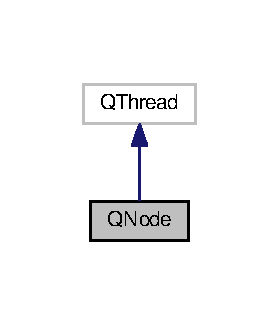
\includegraphics[width=134pt]{class_q_node__inherit__graph}
\end{center}
\end{figure}


Collaboration diagram for Q\+Node\+:
\nopagebreak
\begin{figure}[H]
\begin{center}
\leavevmode
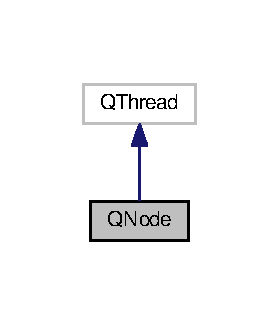
\includegraphics[width=350pt]{class_q_node__coll__graph}
\end{center}
\end{figure}
\subsection*{Signals}
\begin{DoxyCompactItemize}
\item 
void \hyperlink{class_q_node_abddcd4e0187f6d4513bbee7ba4656827}{logging\+Updated} ()
\item 
void \hyperlink{class_q_node_a7888b171c93c5f47334f5d2815adf445}{ros\+Shutdown} ()
\item 
void \hyperlink{class_q_node_a80d139522a1333db2c6ea33914c32378}{write\+On\+Board} (Q\+String)
\end{DoxyCompactItemize}
\subsection*{Public Member Functions}
\begin{DoxyCompactItemize}
\item 
\hyperlink{class_q_node_af26ee8c152283b4a1999dc5d4bd67908}{Q\+Node} (int argc, char $\ast$$\ast$argv, const std\+::string \&name)
\item 
\hyperlink{class_q_node_afed12669e9aed3e70721f507804778ca}{$\sim$\+Q\+Node} ()
\item 
bool \hyperlink{class_q_node_a32d00dbcf15c277e08caabf95af04f6e}{on\+\_\+init} ()
\item 
void \hyperlink{class_q_node_a770568addece696138f515d38408ff5c}{shutdown} ()
\item 
void \hyperlink{class_q_node_ae585b201389c51a177fa5e2fde252c84}{run} ()
\item 
bool \hyperlink{class_q_node_a65f0fc9f27f336150f33b53a7c51d80b}{trigger\+\_\+one\+\_\+shot} (double tf)
\item 
bool \hyperlink{class_q_node_a23bd7e0744ad4c7b5d5464485375bef1}{trigger} (double t\+\_\+cur)
\item 
Q\+String\+List\+Model $\ast$ \hyperlink{class_q_node_a0a6dae02f9e317488095367203fa8a58}{logging\+Model} ()
\item 
const std\+::string \& \hyperlink{class_q_node_ac21ae24311df97ac0e15c97179763b0e}{node\+Name} ()
\item 
void \hyperlink{class_q_node_a2b1b82bfd6e5e6187fe8216ba840bb09}{wpnts\+\_\+init} ()
\end{DoxyCompactItemize}
\subsection*{Public Attributes}
\begin{DoxyCompactItemize}
\item 
\hyperlink{class_target_manager}{Target\+Manager} \hyperlink{class_q_node_adc66765125dfd755d5e7f0c0eb6e6395}{target\+\_\+manager}
\item 
\hyperlink{class_wrapper}{Wrapper} \hyperlink{class_q_node_ad2d828488fb632a008c7d3ee0e1d1fa2}{chaser\+\_\+wrapper}
\item 
string \hyperlink{class_q_node_a0967d1922eeb7e39eedca309c7003d23}{write\+\_\+path}
\item 
bool \hyperlink{class_q_node_a98b08e7704b00df8648f8c08dffe950c}{is\+\_\+connected} = false
\item 
bool \hyperlink{class_q_node_a6ace2d0aa89adecfe699b3f1c3ce0b0f}{is\+\_\+in\+\_\+session} = false
\item 
bool \hyperlink{class_q_node_a9db73b60d8ffd6ac1e64ab5620f2db49}{is\+\_\+said\+\_\+edf} = false
\item 
double \hyperlink{class_q_node_a2893bbeba854c1cc89d2271804325b7b}{button\+\_\+elapsed} =0
\item 
double \hyperlink{class_q_node_ad1f3252201b932fc5d39b4f80349c7e2}{record\+\_\+dt} = 0.\+5
\item 
ros\+::\+Time \hyperlink{class_q_node_a96e6599c14732ded065ae6a5b004f872}{button\+\_\+click\+\_\+time}
\item 
double \hyperlink{class_q_node_a4b5f0a40821fbb176de620cb5a3921f7}{previous\+\_\+elapsed} = 0
\item 
double \hyperlink{class_q_node_a932e8eb11684f38ae2fb3f23639b7c70}{last\+\_\+tigger\+\_\+time} = 0
\item 
double \hyperlink{class_q_node_a7a127726e48aa5bde733d715af7a744c}{simulation\+\_\+end\+\_\+time}
\item 
double \hyperlink{class_q_node_a6e6b7e12d0d9bbc230cc9dc42a2bd087}{early\+\_\+end\+\_\+time} = 0.\+1
\item 
bool \hyperlink{class_q_node_ada91a6275708099206c452df47210045}{arrow\+\_\+record\+\_\+switch} = true
\item 
float \hyperlink{class_q_node_a3430f5db8c773c840b76794c82a9d58f}{pred\+\_\+horizon}
\item 
int \hyperlink{class_q_node_a5d5139bf1420415b2e0c2b0e52db957e}{prediction\+\_\+mode} = 0
\item 
int \hyperlink{class_q_node_aed4571afa880dc86a88b229c6517bfa1}{pred\+\_\+seq} = 4
\end{DoxyCompactItemize}
\subsection*{Protected Member Functions}
\begin{DoxyCompactItemize}
\item 
void \hyperlink{class_q_node_a498b0376fc75702fd8b61b91ef109769}{ros\+\_\+comms\+\_\+init} ()
\end{DoxyCompactItemize}
\subsection*{Protected Attributes}
\begin{DoxyCompactItemize}
\item 
int \hyperlink{class_q_node_aa0c7569195d8b9a6e568e98097f11d52}{init\+\_\+argc}
\item 
char $\ast$$\ast$ \hyperlink{class_q_node_a92c2972e3dd2a5de95d0edf8c75e1e5f}{init\+\_\+argv}
\item 
Q\+String\+List\+Model \hyperlink{class_q_node_aff2207dadd447d4c2554df19b6f7ce48}{logging}
\item 
const std\+::string \hyperlink{class_q_node_ae2a04cf101323be1e9b2be1e63a03b7f}{node\+\_\+name}
\end{DoxyCompactItemize}


\subsection{Detailed Description}


\subsection{Constructor \& Destructor Documentation}
\index{Q\+Node@{Q\+Node}!Q\+Node@{Q\+Node}}
\index{Q\+Node@{Q\+Node}!Q\+Node@{Q\+Node}}
\subsubsection[{\texorpdfstring{Q\+Node(int argc, char $\ast$$\ast$argv, const std\+::string \&name)}{QNode(int argc, char **argv, const std::string &name)}}]{\setlength{\rightskip}{0pt plus 5cm}Q\+Node\+::\+Q\+Node (
\begin{DoxyParamCaption}
\item[{int}]{argc, }
\item[{char $\ast$$\ast$}]{argv, }
\item[{const std\+::string \&}]{name}
\end{DoxyParamCaption}
)}\hypertarget{class_q_node_af26ee8c152283b4a1999dc5d4bd67908}{}\label{class_q_node_af26ee8c152283b4a1999dc5d4bd67908}

\begin{DoxyCode}
3                                                           :
4     \hyperlink{class_q_node_aa0c7569195d8b9a6e568e98097f11d52}{init\_argc}(argc),
5     \hyperlink{class_q_node_a92c2972e3dd2a5de95d0edf8c75e1e5f}{init\_argv}(argv),
6     \hyperlink{class_q_node_ae2a04cf101323be1e9b2be1e63a03b7f}{node\_name}(name)
7     \{
8         
9 \}
\end{DoxyCode}
\index{Q\+Node@{Q\+Node}!````~Q\+Node@{$\sim$\+Q\+Node}}
\index{````~Q\+Node@{$\sim$\+Q\+Node}!Q\+Node@{Q\+Node}}
\subsubsection[{\texorpdfstring{$\sim$\+Q\+Node()}{~QNode()}}]{\setlength{\rightskip}{0pt plus 5cm}Q\+Node\+::$\sim$\+Q\+Node (
\begin{DoxyParamCaption}
{}
\end{DoxyParamCaption}
)}\hypertarget{class_q_node_afed12669e9aed3e70721f507804778ca}{}\label{class_q_node_afed12669e9aed3e70721f507804778ca}

\begin{DoxyCode}
10 \{\}
\end{DoxyCode}


\subsection{Member Function Documentation}
\index{Q\+Node@{Q\+Node}!logging\+Model@{logging\+Model}}
\index{logging\+Model@{logging\+Model}!Q\+Node@{Q\+Node}}
\subsubsection[{\texorpdfstring{logging\+Model()}{loggingModel()}}]{\setlength{\rightskip}{0pt plus 5cm}Q\+String\+List\+Model$\ast$ Q\+Node\+::logging\+Model (
\begin{DoxyParamCaption}
{}
\end{DoxyParamCaption}
)\hspace{0.3cm}{\ttfamily [inline]}}\hypertarget{class_q_node_a0a6dae02f9e317488095367203fa8a58}{}\label{class_q_node_a0a6dae02f9e317488095367203fa8a58}

\begin{DoxyCode}
33 \{ \textcolor{keywordflow}{return} &\hyperlink{class_q_node_aff2207dadd447d4c2554df19b6f7ce48}{logging}; \}
\end{DoxyCode}
\index{Q\+Node@{Q\+Node}!logging\+Updated@{logging\+Updated}}
\index{logging\+Updated@{logging\+Updated}!Q\+Node@{Q\+Node}}
\subsubsection[{\texorpdfstring{logging\+Updated}{loggingUpdated}}]{\setlength{\rightskip}{0pt plus 5cm}void Q\+Node\+::logging\+Updated (
\begin{DoxyParamCaption}
{}
\end{DoxyParamCaption}
)\hspace{0.3cm}{\ttfamily [signal]}}\hypertarget{class_q_node_abddcd4e0187f6d4513bbee7ba4656827}{}\label{class_q_node_abddcd4e0187f6d4513bbee7ba4656827}
\index{Q\+Node@{Q\+Node}!node\+Name@{node\+Name}}
\index{node\+Name@{node\+Name}!Q\+Node@{Q\+Node}}
\subsubsection[{\texorpdfstring{node\+Name()}{nodeName()}}]{\setlength{\rightskip}{0pt plus 5cm}const std\+::string\& Q\+Node\+::node\+Name (
\begin{DoxyParamCaption}
{}
\end{DoxyParamCaption}
)\hspace{0.3cm}{\ttfamily [inline]}}\hypertarget{class_q_node_ac21ae24311df97ac0e15c97179763b0e}{}\label{class_q_node_ac21ae24311df97ac0e15c97179763b0e}

\begin{DoxyCode}
34 \{ \textcolor{keywordflow}{return} \hyperlink{class_q_node_ae2a04cf101323be1e9b2be1e63a03b7f}{node\_name}; \}
\end{DoxyCode}
\index{Q\+Node@{Q\+Node}!on\+\_\+init@{on\+\_\+init}}
\index{on\+\_\+init@{on\+\_\+init}!Q\+Node@{Q\+Node}}
\subsubsection[{\texorpdfstring{on\+\_\+init()}{on_init()}}]{\setlength{\rightskip}{0pt plus 5cm}bool Q\+Node\+::on\+\_\+init (
\begin{DoxyParamCaption}
{}
\end{DoxyParamCaption}
)}\hypertarget{class_q_node_a32d00dbcf15c277e08caabf95af04f6e}{}\label{class_q_node_a32d00dbcf15c277e08caabf95af04f6e}

\begin{DoxyCode}
34                    \{
35 
36     ros::init(\hyperlink{class_q_node_aa0c7569195d8b9a6e568e98097f11d52}{init\_argc},\hyperlink{class_q_node_a92c2972e3dd2a5de95d0edf8c75e1e5f}{init\_argv},\hyperlink{class_q_node_ae2a04cf101323be1e9b2be1e63a03b7f}{node\_name});
37     \textcolor{keywordflow}{if} ( ! ros::master::check() ) \{
38         \textcolor{keywordflow}{return} \textcolor{keyword}{false};
39     \}
40     ros::start(); \textcolor{comment}{// our node handles go out of scope, so we want to control shutdown explicitly.}
41     \hyperlink{class_q_node_a498b0376fc75702fd8b61b91ef109769}{ros\_comms\_init}();
42     start();
43     \textcolor{keywordflow}{return} \textcolor{keyword}{true};
44 \}
\end{DoxyCode}
\index{Q\+Node@{Q\+Node}!ros\+\_\+comms\+\_\+init@{ros\+\_\+comms\+\_\+init}}
\index{ros\+\_\+comms\+\_\+init@{ros\+\_\+comms\+\_\+init}!Q\+Node@{Q\+Node}}
\subsubsection[{\texorpdfstring{ros\+\_\+comms\+\_\+init()}{ros_comms_init()}}]{\setlength{\rightskip}{0pt plus 5cm}void Q\+Node\+::ros\+\_\+comms\+\_\+init (
\begin{DoxyParamCaption}
{}
\end{DoxyParamCaption}
)\hspace{0.3cm}{\ttfamily [protected]}}\hypertarget{class_q_node_a498b0376fc75702fd8b61b91ef109769}{}\label{class_q_node_a498b0376fc75702fd8b61b91ef109769}

\begin{DoxyCode}
11                           \{
12     
13     ros::NodeHandle nh(\textcolor{stringliteral}{"~"});
14     nh.param(\textcolor{stringliteral}{"pred\_horizon"},\hyperlink{class_q_node_a3430f5db8c773c840b76794c82a9d58f}{pred\_horizon},\textcolor{keywordtype}{float}(3.0));
15     nh.param(\textcolor{stringliteral}{"early\_end\_time"},\hyperlink{class_q_node_a6e6b7e12d0d9bbc230cc9dc42a2bd087}{early\_end\_time},0.1);
16     nh.param<\textcolor{keywordtype}{int}>(\textcolor{stringliteral}{"pred\_seq"},\hyperlink{class_q_node_aed4571afa880dc86a88b229c6517bfa1}{pred\_seq},4);
17 
18     \textcolor{comment}{// target manager init}
19     this->\hyperlink{class_q_node_adc66765125dfd755d5e7f0c0eb6e6395}{target\_manager}.\hyperlink{class_target_manager_a293bcb3b559c6e7c4ef549873791f092}{init}(nh);
20 
21     \textcolor{comment}{// wrapper init}
22     this->\hyperlink{class_q_node_ad2d828488fb632a008c7d3ee0e1d1fa2}{chaser\_wrapper}.\hyperlink{class_wrapper_af336781e7d75d525e7b152366a0e0d93}{init}(nh);
23 
24 \}
\end{DoxyCode}
\index{Q\+Node@{Q\+Node}!ros\+Shutdown@{ros\+Shutdown}}
\index{ros\+Shutdown@{ros\+Shutdown}!Q\+Node@{Q\+Node}}
\subsubsection[{\texorpdfstring{ros\+Shutdown}{rosShutdown}}]{\setlength{\rightskip}{0pt plus 5cm}void Q\+Node\+::ros\+Shutdown (
\begin{DoxyParamCaption}
{}
\end{DoxyParamCaption}
)\hspace{0.3cm}{\ttfamily [signal]}}\hypertarget{class_q_node_a7888b171c93c5f47334f5d2815adf445}{}\label{class_q_node_a7888b171c93c5f47334f5d2815adf445}
\index{Q\+Node@{Q\+Node}!run@{run}}
\index{run@{run}!Q\+Node@{Q\+Node}}
\subsubsection[{\texorpdfstring{run()}{run()}}]{\setlength{\rightskip}{0pt plus 5cm}void Q\+Node\+::run (
\begin{DoxyParamCaption}
{}
\end{DoxyParamCaption}
)}\hypertarget{class_q_node_ae585b201389c51a177fa5e2fde252c84}{}\label{class_q_node_ae585b201389c51a177fa5e2fde252c84}

\begin{DoxyCode}
46                \{
47     ros::Rate loop\_rate(50);
48     \hyperlink{class_q_node_a80d139522a1333db2c6ea33914c32378}{writeOnBoard}(\textcolor{stringliteral}{"waiting EDF computation..."});
49 
50     \textcolor{keywordflow}{while}(ros::ok())\{
51         \textcolor{keywordtype}{double} sim\_time;
52         
53         \textcolor{keywordflow}{if}(\hyperlink{class_q_node_a6ace2d0aa89adecfe699b3f1c3ce0b0f}{is\_in\_session})\{ \textcolor{comment}{// activated}
54             \textcolor{comment}{// current simulation time}
55             sim\_time = \hyperlink{class_q_node_a4b5f0a40821fbb176de620cb5a3921f7}{previous\_elapsed} + (ros::Time::now() - 
      \hyperlink{class_q_node_a96e6599c14732ded065ae6a5b004f872}{button\_click\_time}).toSec();
56             
57             \textcolor{comment}{// trigger condition }
58             \textcolor{keywordtype}{bool} trigger\_condition;
59             \textcolor{keywordflow}{if}(\hyperlink{class_q_node_a5d5139bf1420415b2e0c2b0e52db957e}{prediction\_mode} == 0)
60                 trigger\_condition = (\hyperlink{class_q_node_a932e8eb11684f38ae2fb3f23639b7c70}{last\_tigger\_time} == 0 or (sim\_time - 
      \hyperlink{class_q_node_a932e8eb11684f38ae2fb3f23639b7c70}{last\_tigger\_time}) > \hyperlink{class_q_node_a3430f5db8c773c840b76794c82a9d58f}{pred\_horizon} - \hyperlink{class_q_node_a6e6b7e12d0d9bbc230cc9dc42a2bd087}{early\_end\_time} ) and sim\_time 
      <\hyperlink{class_q_node_a7a127726e48aa5bde733d715af7a744c}{simulation\_end\_time};
61             \textcolor{keywordflow}{else} 
62                 trigger\_condition = \textcolor{keyword}{false}; \textcolor{comment}{// TODO for real prediction case }
63 
64             \textcolor{comment}{// if triggered do the followings }
65             \textcolor{keywordflow}{if}(trigger\_condition)                                
66                 \hyperlink{class_q_node_a23bd7e0744ad4c7b5d5464485375bef1}{trigger}(sim\_time);
67             
68        
69         \}\textcolor{keywordflow}{else}
70             sim\_time = \hyperlink{class_q_node_a4b5f0a40821fbb176de620cb5a3921f7}{previous\_elapsed}; 
71         
72         \textcolor{comment}{// session (publish the current information)        }
73         \hyperlink{class_q_node_adc66765125dfd755d5e7f0c0eb6e6395}{target\_manager}.\hyperlink{class_target_manager_a4af88c70bb8a0af0171ee9a49536d5c0}{session}(sim\_time);
74         \hyperlink{class_q_node_ad2d828488fb632a008c7d3ee0e1d1fa2}{chaser\_wrapper}.\hyperlink{class_wrapper_a009ee5c325926f92df42319d5469a376}{session}(sim\_time);
75         
76 
77         \textcolor{comment}{// chaser information board }
78         \textcolor{keywordflow}{if}(\hyperlink{class_q_node_ad2d828488fb632a008c7d3ee0e1d1fa2}{chaser\_wrapper}.\hyperlink{class_wrapper_a8cddd5ffbaeb5ab0b5d8d8d0c74f810f}{objects\_handler}.
      \hyperlink{class_objects_handler_acf1ef1b318defc2a39d87cea72689478}{is\_map\_recieved} and (not \hyperlink{class_q_node_a9db73b60d8ffd6ac1e64ab5620f2db49}{is\_said\_edf}))\{
79             \hyperlink{class_q_node_a80d139522a1333db2c6ea33914c32378}{writeOnBoard}(\textcolor{stringliteral}{"EDF loaded."});
80             is\_said\_edf = \textcolor{keyword}{true};
81         \}
82         
83         ros::spinOnce();
84         loop\_rate.sleep();
85     \}
86 
87 
88     Q\_EMIT \hyperlink{class_q_node_a7888b171c93c5f47334f5d2815adf445}{rosShutdown}();
89 
90 \}
\end{DoxyCode}
\index{Q\+Node@{Q\+Node}!shutdown@{shutdown}}
\index{shutdown@{shutdown}!Q\+Node@{Q\+Node}}
\subsubsection[{\texorpdfstring{shutdown()}{shutdown()}}]{\setlength{\rightskip}{0pt plus 5cm}void Q\+Node\+::shutdown (
\begin{DoxyParamCaption}
{}
\end{DoxyParamCaption}
)}\hypertarget{class_q_node_a770568addece696138f515d38408ff5c}{}\label{class_q_node_a770568addece696138f515d38408ff5c}

\begin{DoxyCode}
26                      \{
27     \textcolor{keywordflow}{if}(ros::isStarted()) \{
28       ros::shutdown(); \textcolor{comment}{// explicitly needed since we use ros::start();}
29       ros::waitForShutdown();
30     \}
31     wait();
32 \}
\end{DoxyCode}
\index{Q\+Node@{Q\+Node}!trigger@{trigger}}
\index{trigger@{trigger}!Q\+Node@{Q\+Node}}
\subsubsection[{\texorpdfstring{trigger(double t\+\_\+cur)}{trigger(double t_cur)}}]{\setlength{\rightskip}{0pt plus 5cm}bool Q\+Node\+::trigger (
\begin{DoxyParamCaption}
\item[{double}]{t\+\_\+cur}
\end{DoxyParamCaption}
)}\hypertarget{class_q_node_a23bd7e0744ad4c7b5d5464485375bef1}{}\label{class_q_node_a23bd7e0744ad4c7b5d5464485375bef1}

\begin{DoxyCode}
118                                \{
119 
120     \hyperlink{class_q_node_a932e8eb11684f38ae2fb3f23639b7c70}{last\_tigger\_time} = t\_cur;
121     VectorXd pred\_horizon\_vec(\hyperlink{class_q_node_aed4571afa880dc86a88b229c6517bfa1}{pred\_seq});
122     pred\_horizon\_vec.setLinSpaced(\hyperlink{class_q_node_aed4571afa880dc86a88b229c6517bfa1}{pred\_seq},t\_cur,t\_cur + \hyperlink{class_q_node_a3430f5db8c773c840b76794c82a9d58f}{pred\_horizon}); 
123     \textcolor{comment}{// if(t\_cur + pred\_horizon > simulation\_end\_time)\{}
124 
125     \textcolor{comment}{//     cout<<"almost there"<<endl;}
126     \textcolor{comment}{// \}}
127     \textcolor{comment}{// pred\_horizon\_vec = pred\_horizon\_vec.cwiseMin(simulation\_end\_time); // clamping with final time}
128     cout<<\textcolor{stringliteral}{"current horizon vector:\(\backslash\)n"}<<pred\_horizon\_vec<<endl; 
129     \textcolor{comment}{// we chase under this prediction }
130     vector<Point> target\_seq = \hyperlink{class_q_node_adc66765125dfd755d5e7f0c0eb6e6395}{target\_manager}.\hyperlink{class_target_manager_a63bbc724844890316a654380d0354e93}{eval\_time\_seq}(pred\_horizon\_vec);
131     
132     \textcolor{keywordflow}{if} (target\_seq.size() == 0)\{
133         this->\hyperlink{class_q_node_a80d139522a1333db2c6ea33914c32378}{writeOnBoard}(\textcolor{stringliteral}{"size of provided target sequence is zero. please generate target
       traj first."});
134         \textcolor{keywordflow}{return} \textcolor{keyword}{false};
135     \}
136     \textcolor{keywordflow}{if}(not \hyperlink{class_q_node_ad2d828488fb632a008c7d3ee0e1d1fa2}{chaser\_wrapper}.\hyperlink{class_wrapper_a8cddd5ffbaeb5ab0b5d8d8d0c74f810f}{objects\_handler}.
      \hyperlink{class_objects_handler_a16165ae7c0167ba8d2a0151a8a4fbfd5}{is\_chaser\_spawned})\{
137         this->\hyperlink{class_q_node_a80d139522a1333db2c6ea33914c32378}{writeOnBoard}(\textcolor{stringliteral}{"chaser has not been spawned."});
138         \textcolor{keywordflow}{return} \textcolor{keyword}{false};
139     \}
140 
141     \textcolor{keywordflow}{if}(not \hyperlink{class_q_node_ad2d828488fb632a008c7d3ee0e1d1fa2}{chaser\_wrapper}.\hyperlink{class_wrapper_a8cddd5ffbaeb5ab0b5d8d8d0c74f810f}{objects\_handler}.
      \hyperlink{class_objects_handler_acf1ef1b318defc2a39d87cea72689478}{is\_map\_recieved})\{
142         this->\hyperlink{class_q_node_a80d139522a1333db2c6ea33914c32378}{writeOnBoard}(\textcolor{stringliteral}{"octomap or edf has not been uploaded."});
143         \textcolor{keywordflow}{return} \textcolor{keyword}{false};
144     \}    
145 
146 
147     \textcolor{keywordflow}{return} \hyperlink{class_q_node_ad2d828488fb632a008c7d3ee0e1d1fa2}{chaser\_wrapper}.\hyperlink{class_wrapper_a21a0e115ea80e053e4f2defd1362b92f}{trigger\_chasing}(target\_seq,pred\_horizon\_vec); 
148 \}\end{DoxyCode}
\index{Q\+Node@{Q\+Node}!trigger\+\_\+one\+\_\+shot@{trigger\+\_\+one\+\_\+shot}}
\index{trigger\+\_\+one\+\_\+shot@{trigger\+\_\+one\+\_\+shot}!Q\+Node@{Q\+Node}}
\subsubsection[{\texorpdfstring{trigger\+\_\+one\+\_\+shot(double tf)}{trigger_one_shot(double tf)}}]{\setlength{\rightskip}{0pt plus 5cm}bool Q\+Node\+::trigger\+\_\+one\+\_\+shot (
\begin{DoxyParamCaption}
\item[{double}]{tf}
\end{DoxyParamCaption}
)}\hypertarget{class_q_node_a65f0fc9f27f336150f33b53a7c51d80b}{}\label{class_q_node_a65f0fc9f27f336150f33b53a7c51d80b}

\begin{DoxyCode}
92                                      \{
93     
94 
95 
96     \textcolor{comment}{// target global waypoitns  }
97     vector<Point> target\_seq = \hyperlink{_common_8h_a81915b091c29bc9aef6a74ab374f479a}{extract\_pnts\_from\_path}(
      \hyperlink{class_q_node_adc66765125dfd755d5e7f0c0eb6e6395}{target\_manager}.\hyperlink{class_target_manager_a747b82bf5cb4d1d3574dbc08a117538f}{get\_global\_waypoints}());
98     \textcolor{keywordflow}{if} (target\_seq.size() == 0)\{
99         this->\hyperlink{class_q_node_a80d139522a1333db2c6ea33914c32378}{writeOnBoard}(\textcolor{stringliteral}{"size of provided target sequence is zero. please generate target
       traj first."});
100         \textcolor{keywordflow}{return} \textcolor{keyword}{false};
101     \}
102     \textcolor{keywordflow}{if}(not \hyperlink{class_q_node_ad2d828488fb632a008c7d3ee0e1d1fa2}{chaser\_wrapper}.\hyperlink{class_wrapper_a8cddd5ffbaeb5ab0b5d8d8d0c74f810f}{objects\_handler}.
      \hyperlink{class_objects_handler_a16165ae7c0167ba8d2a0151a8a4fbfd5}{is\_chaser\_spawned})\{
103         this->\hyperlink{class_q_node_a80d139522a1333db2c6ea33914c32378}{writeOnBoard}(\textcolor{stringliteral}{"chaser has not been spawned."});
104         \textcolor{keywordflow}{return} \textcolor{keyword}{false};
105     \}
106 
107     \textcolor{keywordflow}{if}(not \hyperlink{class_q_node_ad2d828488fb632a008c7d3ee0e1d1fa2}{chaser\_wrapper}.\hyperlink{class_wrapper_a8cddd5ffbaeb5ab0b5d8d8d0c74f810f}{objects\_handler}.
      \hyperlink{class_objects_handler_acf1ef1b318defc2a39d87cea72689478}{is\_map\_recieved})\{
108         this->\hyperlink{class_q_node_a80d139522a1333db2c6ea33914c32378}{writeOnBoard}(\textcolor{stringliteral}{"octomap or edf has not been uploaded."});
109         \textcolor{keywordflow}{return} \textcolor{keyword}{false};
110     \}    
111 
112     \textcolor{comment}{// trigger chasing}
113     VectorXd knots;    
114     knots.setLinSpaced(\hyperlink{class_q_node_adc66765125dfd755d5e7f0c0eb6e6395}{target\_manager}.\hyperlink{class_target_manager_a0bbcb1981504e3bc587c3a98f41a91e9}{queue}.size(),0,tf); 
115     \textcolor{keywordtype}{bool} is\_success =  \hyperlink{class_q_node_ad2d828488fb632a008c7d3ee0e1d1fa2}{chaser\_wrapper}.\hyperlink{class_wrapper_a21a0e115ea80e053e4f2defd1362b92f}{trigger\_chasing}(target\_seq,knots);      
        
116 \}
\end{DoxyCode}
\index{Q\+Node@{Q\+Node}!wpnts\+\_\+init@{wpnts\+\_\+init}}
\index{wpnts\+\_\+init@{wpnts\+\_\+init}!Q\+Node@{Q\+Node}}
\subsubsection[{\texorpdfstring{wpnts\+\_\+init()}{wpnts_init()}}]{\setlength{\rightskip}{0pt plus 5cm}void Q\+Node\+::wpnts\+\_\+init (
\begin{DoxyParamCaption}
{}
\end{DoxyParamCaption}
)}\hypertarget{class_q_node_a2b1b82bfd6e5e6187fe8216ba840bb09}{}\label{class_q_node_a2b1b82bfd6e5e6187fe8216ba840bb09}
\index{Q\+Node@{Q\+Node}!write\+On\+Board@{write\+On\+Board}}
\index{write\+On\+Board@{write\+On\+Board}!Q\+Node@{Q\+Node}}
\subsubsection[{\texorpdfstring{write\+On\+Board}{writeOnBoard}}]{\setlength{\rightskip}{0pt plus 5cm}void Q\+Node\+::write\+On\+Board (
\begin{DoxyParamCaption}
\item[{Q\+String}]{}
\end{DoxyParamCaption}
)\hspace{0.3cm}{\ttfamily [signal]}}\hypertarget{class_q_node_a80d139522a1333db2c6ea33914c32378}{}\label{class_q_node_a80d139522a1333db2c6ea33914c32378}


\subsection{Member Data Documentation}
\index{Q\+Node@{Q\+Node}!arrow\+\_\+record\+\_\+switch@{arrow\+\_\+record\+\_\+switch}}
\index{arrow\+\_\+record\+\_\+switch@{arrow\+\_\+record\+\_\+switch}!Q\+Node@{Q\+Node}}
\subsubsection[{\texorpdfstring{arrow\+\_\+record\+\_\+switch}{arrow_record_switch}}]{\setlength{\rightskip}{0pt plus 5cm}bool Q\+Node\+::arrow\+\_\+record\+\_\+switch = true}\hypertarget{class_q_node_ada91a6275708099206c452df47210045}{}\label{class_q_node_ada91a6275708099206c452df47210045}
\index{Q\+Node@{Q\+Node}!button\+\_\+click\+\_\+time@{button\+\_\+click\+\_\+time}}
\index{button\+\_\+click\+\_\+time@{button\+\_\+click\+\_\+time}!Q\+Node@{Q\+Node}}
\subsubsection[{\texorpdfstring{button\+\_\+click\+\_\+time}{button_click_time}}]{\setlength{\rightskip}{0pt plus 5cm}ros\+::\+Time Q\+Node\+::button\+\_\+click\+\_\+time}\hypertarget{class_q_node_a96e6599c14732ded065ae6a5b004f872}{}\label{class_q_node_a96e6599c14732ded065ae6a5b004f872}
\index{Q\+Node@{Q\+Node}!button\+\_\+elapsed@{button\+\_\+elapsed}}
\index{button\+\_\+elapsed@{button\+\_\+elapsed}!Q\+Node@{Q\+Node}}
\subsubsection[{\texorpdfstring{button\+\_\+elapsed}{button_elapsed}}]{\setlength{\rightskip}{0pt plus 5cm}double Q\+Node\+::button\+\_\+elapsed =0}\hypertarget{class_q_node_a2893bbeba854c1cc89d2271804325b7b}{}\label{class_q_node_a2893bbeba854c1cc89d2271804325b7b}
\index{Q\+Node@{Q\+Node}!chaser\+\_\+wrapper@{chaser\+\_\+wrapper}}
\index{chaser\+\_\+wrapper@{chaser\+\_\+wrapper}!Q\+Node@{Q\+Node}}
\subsubsection[{\texorpdfstring{chaser\+\_\+wrapper}{chaser_wrapper}}]{\setlength{\rightskip}{0pt plus 5cm}{\bf Wrapper} Q\+Node\+::chaser\+\_\+wrapper}\hypertarget{class_q_node_ad2d828488fb632a008c7d3ee0e1d1fa2}{}\label{class_q_node_ad2d828488fb632a008c7d3ee0e1d1fa2}
\index{Q\+Node@{Q\+Node}!early\+\_\+end\+\_\+time@{early\+\_\+end\+\_\+time}}
\index{early\+\_\+end\+\_\+time@{early\+\_\+end\+\_\+time}!Q\+Node@{Q\+Node}}
\subsubsection[{\texorpdfstring{early\+\_\+end\+\_\+time}{early_end_time}}]{\setlength{\rightskip}{0pt plus 5cm}double Q\+Node\+::early\+\_\+end\+\_\+time = 0.\+1}\hypertarget{class_q_node_a6e6b7e12d0d9bbc230cc9dc42a2bd087}{}\label{class_q_node_a6e6b7e12d0d9bbc230cc9dc42a2bd087}
\index{Q\+Node@{Q\+Node}!init\+\_\+argc@{init\+\_\+argc}}
\index{init\+\_\+argc@{init\+\_\+argc}!Q\+Node@{Q\+Node}}
\subsubsection[{\texorpdfstring{init\+\_\+argc}{init_argc}}]{\setlength{\rightskip}{0pt plus 5cm}int Q\+Node\+::init\+\_\+argc\hspace{0.3cm}{\ttfamily [protected]}}\hypertarget{class_q_node_aa0c7569195d8b9a6e568e98097f11d52}{}\label{class_q_node_aa0c7569195d8b9a6e568e98097f11d52}
\index{Q\+Node@{Q\+Node}!init\+\_\+argv@{init\+\_\+argv}}
\index{init\+\_\+argv@{init\+\_\+argv}!Q\+Node@{Q\+Node}}
\subsubsection[{\texorpdfstring{init\+\_\+argv}{init_argv}}]{\setlength{\rightskip}{0pt plus 5cm}char$\ast$$\ast$ Q\+Node\+::init\+\_\+argv\hspace{0.3cm}{\ttfamily [protected]}}\hypertarget{class_q_node_a92c2972e3dd2a5de95d0edf8c75e1e5f}{}\label{class_q_node_a92c2972e3dd2a5de95d0edf8c75e1e5f}
\index{Q\+Node@{Q\+Node}!is\+\_\+connected@{is\+\_\+connected}}
\index{is\+\_\+connected@{is\+\_\+connected}!Q\+Node@{Q\+Node}}
\subsubsection[{\texorpdfstring{is\+\_\+connected}{is_connected}}]{\setlength{\rightskip}{0pt plus 5cm}bool Q\+Node\+::is\+\_\+connected = false}\hypertarget{class_q_node_a98b08e7704b00df8648f8c08dffe950c}{}\label{class_q_node_a98b08e7704b00df8648f8c08dffe950c}
\index{Q\+Node@{Q\+Node}!is\+\_\+in\+\_\+session@{is\+\_\+in\+\_\+session}}
\index{is\+\_\+in\+\_\+session@{is\+\_\+in\+\_\+session}!Q\+Node@{Q\+Node}}
\subsubsection[{\texorpdfstring{is\+\_\+in\+\_\+session}{is_in_session}}]{\setlength{\rightskip}{0pt plus 5cm}bool Q\+Node\+::is\+\_\+in\+\_\+session = false}\hypertarget{class_q_node_a6ace2d0aa89adecfe699b3f1c3ce0b0f}{}\label{class_q_node_a6ace2d0aa89adecfe699b3f1c3ce0b0f}
\index{Q\+Node@{Q\+Node}!is\+\_\+said\+\_\+edf@{is\+\_\+said\+\_\+edf}}
\index{is\+\_\+said\+\_\+edf@{is\+\_\+said\+\_\+edf}!Q\+Node@{Q\+Node}}
\subsubsection[{\texorpdfstring{is\+\_\+said\+\_\+edf}{is_said_edf}}]{\setlength{\rightskip}{0pt plus 5cm}bool Q\+Node\+::is\+\_\+said\+\_\+edf = false}\hypertarget{class_q_node_a9db73b60d8ffd6ac1e64ab5620f2db49}{}\label{class_q_node_a9db73b60d8ffd6ac1e64ab5620f2db49}
\index{Q\+Node@{Q\+Node}!last\+\_\+tigger\+\_\+time@{last\+\_\+tigger\+\_\+time}}
\index{last\+\_\+tigger\+\_\+time@{last\+\_\+tigger\+\_\+time}!Q\+Node@{Q\+Node}}
\subsubsection[{\texorpdfstring{last\+\_\+tigger\+\_\+time}{last_tigger_time}}]{\setlength{\rightskip}{0pt plus 5cm}double Q\+Node\+::last\+\_\+tigger\+\_\+time = 0}\hypertarget{class_q_node_a932e8eb11684f38ae2fb3f23639b7c70}{}\label{class_q_node_a932e8eb11684f38ae2fb3f23639b7c70}
\index{Q\+Node@{Q\+Node}!logging@{logging}}
\index{logging@{logging}!Q\+Node@{Q\+Node}}
\subsubsection[{\texorpdfstring{logging}{logging}}]{\setlength{\rightskip}{0pt plus 5cm}Q\+String\+List\+Model Q\+Node\+::logging\hspace{0.3cm}{\ttfamily [protected]}}\hypertarget{class_q_node_aff2207dadd447d4c2554df19b6f7ce48}{}\label{class_q_node_aff2207dadd447d4c2554df19b6f7ce48}
\index{Q\+Node@{Q\+Node}!node\+\_\+name@{node\+\_\+name}}
\index{node\+\_\+name@{node\+\_\+name}!Q\+Node@{Q\+Node}}
\subsubsection[{\texorpdfstring{node\+\_\+name}{node_name}}]{\setlength{\rightskip}{0pt plus 5cm}const std\+::string Q\+Node\+::node\+\_\+name\hspace{0.3cm}{\ttfamily [protected]}}\hypertarget{class_q_node_ae2a04cf101323be1e9b2be1e63a03b7f}{}\label{class_q_node_ae2a04cf101323be1e9b2be1e63a03b7f}
\index{Q\+Node@{Q\+Node}!pred\+\_\+horizon@{pred\+\_\+horizon}}
\index{pred\+\_\+horizon@{pred\+\_\+horizon}!Q\+Node@{Q\+Node}}
\subsubsection[{\texorpdfstring{pred\+\_\+horizon}{pred_horizon}}]{\setlength{\rightskip}{0pt plus 5cm}float Q\+Node\+::pred\+\_\+horizon}\hypertarget{class_q_node_a3430f5db8c773c840b76794c82a9d58f}{}\label{class_q_node_a3430f5db8c773c840b76794c82a9d58f}
\index{Q\+Node@{Q\+Node}!pred\+\_\+seq@{pred\+\_\+seq}}
\index{pred\+\_\+seq@{pred\+\_\+seq}!Q\+Node@{Q\+Node}}
\subsubsection[{\texorpdfstring{pred\+\_\+seq}{pred_seq}}]{\setlength{\rightskip}{0pt plus 5cm}int Q\+Node\+::pred\+\_\+seq = 4}\hypertarget{class_q_node_aed4571afa880dc86a88b229c6517bfa1}{}\label{class_q_node_aed4571afa880dc86a88b229c6517bfa1}
\index{Q\+Node@{Q\+Node}!prediction\+\_\+mode@{prediction\+\_\+mode}}
\index{prediction\+\_\+mode@{prediction\+\_\+mode}!Q\+Node@{Q\+Node}}
\subsubsection[{\texorpdfstring{prediction\+\_\+mode}{prediction_mode}}]{\setlength{\rightskip}{0pt plus 5cm}int Q\+Node\+::prediction\+\_\+mode = 0}\hypertarget{class_q_node_a5d5139bf1420415b2e0c2b0e52db957e}{}\label{class_q_node_a5d5139bf1420415b2e0c2b0e52db957e}
\index{Q\+Node@{Q\+Node}!previous\+\_\+elapsed@{previous\+\_\+elapsed}}
\index{previous\+\_\+elapsed@{previous\+\_\+elapsed}!Q\+Node@{Q\+Node}}
\subsubsection[{\texorpdfstring{previous\+\_\+elapsed}{previous_elapsed}}]{\setlength{\rightskip}{0pt plus 5cm}double Q\+Node\+::previous\+\_\+elapsed = 0}\hypertarget{class_q_node_a4b5f0a40821fbb176de620cb5a3921f7}{}\label{class_q_node_a4b5f0a40821fbb176de620cb5a3921f7}
\index{Q\+Node@{Q\+Node}!record\+\_\+dt@{record\+\_\+dt}}
\index{record\+\_\+dt@{record\+\_\+dt}!Q\+Node@{Q\+Node}}
\subsubsection[{\texorpdfstring{record\+\_\+dt}{record_dt}}]{\setlength{\rightskip}{0pt plus 5cm}double Q\+Node\+::record\+\_\+dt = 0.\+5}\hypertarget{class_q_node_ad1f3252201b932fc5d39b4f80349c7e2}{}\label{class_q_node_ad1f3252201b932fc5d39b4f80349c7e2}
\index{Q\+Node@{Q\+Node}!simulation\+\_\+end\+\_\+time@{simulation\+\_\+end\+\_\+time}}
\index{simulation\+\_\+end\+\_\+time@{simulation\+\_\+end\+\_\+time}!Q\+Node@{Q\+Node}}
\subsubsection[{\texorpdfstring{simulation\+\_\+end\+\_\+time}{simulation_end_time}}]{\setlength{\rightskip}{0pt plus 5cm}double Q\+Node\+::simulation\+\_\+end\+\_\+time}\hypertarget{class_q_node_a7a127726e48aa5bde733d715af7a744c}{}\label{class_q_node_a7a127726e48aa5bde733d715af7a744c}
\index{Q\+Node@{Q\+Node}!target\+\_\+manager@{target\+\_\+manager}}
\index{target\+\_\+manager@{target\+\_\+manager}!Q\+Node@{Q\+Node}}
\subsubsection[{\texorpdfstring{target\+\_\+manager}{target_manager}}]{\setlength{\rightskip}{0pt plus 5cm}{\bf Target\+Manager} Q\+Node\+::target\+\_\+manager}\hypertarget{class_q_node_adc66765125dfd755d5e7f0c0eb6e6395}{}\label{class_q_node_adc66765125dfd755d5e7f0c0eb6e6395}
\index{Q\+Node@{Q\+Node}!write\+\_\+path@{write\+\_\+path}}
\index{write\+\_\+path@{write\+\_\+path}!Q\+Node@{Q\+Node}}
\subsubsection[{\texorpdfstring{write\+\_\+path}{write_path}}]{\setlength{\rightskip}{0pt plus 5cm}string Q\+Node\+::write\+\_\+path}\hypertarget{class_q_node_a0967d1922eeb7e39eedca309c7003d23}{}\label{class_q_node_a0967d1922eeb7e39eedca309c7003d23}


The documentation for this class was generated from the following files\+:\begin{DoxyCompactItemize}
\item 
src/qt\+\_\+ui/\hyperlink{qnode_8h}{qnode.\+h}\item 
src/qt\+\_\+ui/\hyperlink{qnode_8cpp}{qnode.\+cpp}\end{DoxyCompactItemize}

\hypertarget{class_ui___main_window}{}\section{Ui\+\_\+\+Main\+Window Class Reference}
\label{class_ui___main_window}\index{Ui\+\_\+\+Main\+Window@{Ui\+\_\+\+Main\+Window}}


Inheritance diagram for Ui\+\_\+\+Main\+Window\+:\nopagebreak
\begin{figure}[H]
\begin{center}
\leavevmode
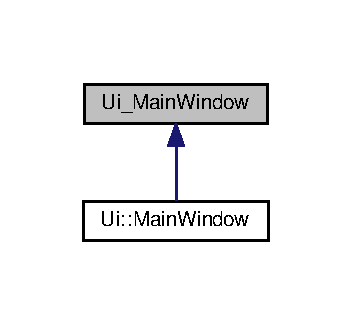
\includegraphics[width=169pt]{class_ui___main_window__inherit__graph}
\end{center}
\end{figure}
\subsection*{Public Member Functions}
\begin{DoxyCompactItemize}
\item 
void {\bfseries setup\+Ui} (Q\+Main\+Window $\ast$\hyperlink{class_main_window}{Main\+Window})\hypertarget{class_ui___main_window_acf4a0872c4c77d8f43a2ec66ed849b58}{}\label{class_ui___main_window_acf4a0872c4c77d8f43a2ec66ed849b58}

\item 
void {\bfseries retranslate\+Ui} (Q\+Main\+Window $\ast$\hyperlink{class_main_window}{Main\+Window})\hypertarget{class_ui___main_window_a097dd160c3534a204904cb374412c618}{}\label{class_ui___main_window_a097dd160c3534a204904cb374412c618}

\end{DoxyCompactItemize}
\subsection*{Public Attributes}
\begin{DoxyCompactItemize}
\item 
Q\+Widget $\ast$ {\bfseries central\+Widget}\hypertarget{class_ui___main_window_a30075506c2116c3ed4ff25e07ae75f81}{}\label{class_ui___main_window_a30075506c2116c3ed4ff25e07ae75f81}

\item 
Q\+Label $\ast$ {\bfseries label\+\_\+larr}\hypertarget{class_ui___main_window_a32587f1e879f5b685d375d2daa20f7a6}{}\label{class_ui___main_window_a32587f1e879f5b685d375d2daa20f7a6}

\item 
Q\+Label $\ast$ {\bfseries label\+\_\+larr2}\hypertarget{class_ui___main_window_a06fc1a01ac3ba3d4d1f75a0e8ab06684}{}\label{class_ui___main_window_a06fc1a01ac3ba3d4d1f75a0e8ab06684}

\item 
Q\+Label $\ast$ {\bfseries label}\hypertarget{class_ui___main_window_ad9c89133780f28e6efa2ec17ceb9cff5}{}\label{class_ui___main_window_ad9c89133780f28e6efa2ec17ceb9cff5}

\item 
Q\+Push\+Button $\ast$ {\bfseries push\+Button\+\_\+ros}\hypertarget{class_ui___main_window_a2667c2b4f9c61bf9895b73d07d4b5172}{}\label{class_ui___main_window_a2667c2b4f9c61bf9895b73d07d4b5172}

\item 
Q\+Push\+Button $\ast$ {\bfseries push\+Button\+\_\+waypoint}\hypertarget{class_ui___main_window_a6b5d7c0f96cdb3276a33746fbcd7e8c7}{}\label{class_ui___main_window_a6b5d7c0f96cdb3276a33746fbcd7e8c7}

\item 
Q\+Push\+Button $\ast$ {\bfseries push\+Button\+\_\+trajectory}\hypertarget{class_ui___main_window_a9d644554288462450d209192c1998095}{}\label{class_ui___main_window_a9d644554288462450d209192c1998095}

\item 
Q\+Push\+Button $\ast$ {\bfseries push\+Button\+\_\+simulation}\hypertarget{class_ui___main_window_afd109ead0ad1ae7ae67ad1df803c9c38}{}\label{class_ui___main_window_afd109ead0ad1ae7ae67ad1df803c9c38}

\item 
Q\+Text\+Edit $\ast$ {\bfseries text\+Edit\+\_\+board}\hypertarget{class_ui___main_window_af13441b9fd874f1aeb2ec5cefaeb0bce}{}\label{class_ui___main_window_af13441b9fd874f1aeb2ec5cefaeb0bce}

\item 
Q\+Push\+Button $\ast$ {\bfseries push\+Button\+\_\+save}\hypertarget{class_ui___main_window_a257d4df0fe652a526e4fddba93c7a7d8}{}\label{class_ui___main_window_a257d4df0fe652a526e4fddba93c7a7d8}

\item 
Q\+Line\+Edit $\ast$ {\bfseries line\+Edit\+\_\+logging\+\_\+dir}\hypertarget{class_ui___main_window_a7ab71242b81ef9d13f83c16f6328f35d}{}\label{class_ui___main_window_a7ab71242b81ef9d13f83c16f6328f35d}

\item 
Q\+Label $\ast$ {\bfseries label\+\_\+2}\hypertarget{class_ui___main_window_a2e2516d755e4dd53fc905dabddf2738a}{}\label{class_ui___main_window_a2e2516d755e4dd53fc905dabddf2738a}

\item 
Q\+Label $\ast$ {\bfseries label\+\_\+3}\hypertarget{class_ui___main_window_a0376fd90247280e7c7957cc70628708c}{}\label{class_ui___main_window_a0376fd90247280e7c7957cc70628708c}

\item 
Q\+Line\+Edit $\ast$ {\bfseries line\+Edit\+\_\+target\+\_\+trajectory}\hypertarget{class_ui___main_window_a4a75bfb754049f89fccef822cad712d6}{}\label{class_ui___main_window_a4a75bfb754049f89fccef822cad712d6}

\item 
Q\+Push\+Button $\ast$ {\bfseries push\+Button\+\_\+load}\hypertarget{class_ui___main_window_a67832089879377ce16b3f26fbb2cc3f2}{}\label{class_ui___main_window_a67832089879377ce16b3f26fbb2cc3f2}

\item 
Q\+Push\+Button $\ast$ {\bfseries push\+Button\+\_\+clear}\hypertarget{class_ui___main_window_a5d7af3b0fdbc605e3fd8ae6ceffa0d29}{}\label{class_ui___main_window_a5d7af3b0fdbc605e3fd8ae6ceffa0d29}

\item 
Q\+Push\+Button $\ast$ {\bfseries push\+Button\+\_\+undo}\hypertarget{class_ui___main_window_ab3fd048b1a1dee328d8e1b433955bf29}{}\label{class_ui___main_window_ab3fd048b1a1dee328d8e1b433955bf29}

\item 
Q\+Label $\ast$ {\bfseries label\+\_\+4}\hypertarget{class_ui___main_window_a78c7e10730b43c6700cd7216911ed76a}{}\label{class_ui___main_window_a78c7e10730b43c6700cd7216911ed76a}

\item 
Q\+Line\+Edit $\ast$ {\bfseries line\+Edit\+\_\+tf}\hypertarget{class_ui___main_window_afc0d94ce5096c619c413cfae9b62014c}{}\label{class_ui___main_window_afc0d94ce5096c619c413cfae9b62014c}

\item 
Q\+Push\+Button $\ast$ {\bfseries push\+Button\+\_\+chaser}\hypertarget{class_ui___main_window_a9e8499b7c9a9717499abde993da72ed5}{}\label{class_ui___main_window_a9e8499b7c9a9717499abde993da72ed5}

\item 
Q\+Menu\+Bar $\ast$ {\bfseries menu\+Bar}\hypertarget{class_ui___main_window_a2be1c24ec9adfca18e1dcc951931457f}{}\label{class_ui___main_window_a2be1c24ec9adfca18e1dcc951931457f}

\item 
Q\+Menu $\ast$ {\bfseries menu\+Auto\+\_\+chaser}\hypertarget{class_ui___main_window_a8946bc17fa5b33e1c89ef82fdacab1d8}{}\label{class_ui___main_window_a8946bc17fa5b33e1c89ef82fdacab1d8}

\item 
Q\+Tool\+Bar $\ast$ {\bfseries main\+Tool\+Bar}\hypertarget{class_ui___main_window_a5172877001c8c7b4e0f6de50421867d1}{}\label{class_ui___main_window_a5172877001c8c7b4e0f6de50421867d1}

\item 
Q\+Status\+Bar $\ast$ {\bfseries status\+Bar}\hypertarget{class_ui___main_window_a50fa481337604bcc8bf68de18ab16ecd}{}\label{class_ui___main_window_a50fa481337604bcc8bf68de18ab16ecd}

\end{DoxyCompactItemize}


The documentation for this class was generated from the following file\+:\begin{DoxyCompactItemize}
\item 
src/build-\/qt\+\_\+ui-\/\+Desktop-\/\+Debug/ui\+\_\+mainwindow.\+h\end{DoxyCompactItemize}

%--- End generated contents ---

% Index
\backmatter
\newpage
\phantomsection
\clearemptydoublepage
\addcontentsline{toc}{chapter}{Index}
\printindex

\end{document}
